\documentclass[report,dvipdfmx]{jlreq}
\usepackage{graphicx}
\usepackage[version=4]{mhchem}
\usepackage{cite}
\usepackage{amsmath}
\usepackage{mathtools}
\usepackage{textcomp}
% \usepackage{caption}
\usepackage{subcaption}
% \usepackage{amssymb}
\usepackage{url}
% \usepackage{hyperref}
% \usepackage{pxjahyper}

\includeonly{
    master_thesis_contents/0abstract.tex,
    master_thesis_contents/1intro.tex,
    master_thesis_contents/2mmobs.tex,
    master_thesis_contents/3mm_analysis.tex,
    master_thesis_contents/4results.tex,
    master_thesis_contents/5discussion.tex,
    master_thesis_contents/6conclusion.tex,
    master_thesis_contents/7ack.tex,
    master_thesis_contents/app1sofie.tex,
    master_thesis_contents/app2poes.tex,
}

\begin{document}

\title{ミリ波分光計を用いた北極域・南極域における \\ 中層大気中の一酸化窒素分子変動の観測的研究}
\author{名古屋大学大学院工学研究科電気工学専攻 \\ 後藤宏文}
\date{\empty}

\maketitle

% abstract
\begin{abstract}
    我々のグループは、太陽活動に伴って極域に降り込む高エネルギー粒子が$\mathrm{NO}_x$(窒素酸化物)やオゾンなどの中層大気中の微量分子に及ぼす影響を観測的に調べるため、2012年から南極・昭和基地(69.00\textdegree S, 39.85\textdegree E)、2016年から北極域のノルウェー・トロムソ(69.35\textdegree N, 19.14\textdegree E)でミリ波分光観測を行っている。
    先行研究(Isono et al., 2014)では、ミリ波分光を用いた昭和基地でのNO(一酸化窒素)のモニタリング観測において、季節変化に伴う長期変動の他、冬期に高エネルギー粒子の影響によると考えられる短期変動が確認された。
    しかし、夏期は高エネルギー粒子の影響だけでなく、太陽光での光解離による減少もあり、これらを切り分けることができなかった。
    そこで本研究では、季節が逆転する北半球の極域にも着目し、両極域での同時観測を実現するために、解析に用いることができるかデータを精査し柱密度の導出を行った。
    導出した\ce{NO}の柱密度の時間変動について、高エネルギー粒子がどのように影響を与えているかを調べた。
    \par
    昭和基地とトロムソでは、ミリ波分光計の仕様は異なっている。
    トロムソでは$1.0\ \mathrm{GHz}$の帯域を持つFFT分光計を使い\ce{NO}の2本の超微細構造線のスペクトルを同時観測しているが、昭和基地の分光計帯域は$2.5\ \mathrm{GHz}$であり、6本のスペクトルの同時観測が可能である。
    \par
    本研究では、これらのスペクトルデータの解析手法を検討した後、トロムソについては2018年12月26日から2019年3月10日までの75日間、昭和基地については2023年3月22日から31日までの10日間にわたる\ce{NO}の観測データの中から\ce{NO}の柱密度の導出を行って、その変動について考察した。
    \par
    トロムソの分光計では積分時間は24時間であったが、\ce{NO}の6本の超微細構造線から導出される柱密度を平均することで、昭和基地における積分時間は12時間と短くした。
    昭和基地での柱密度の誤差の平均はトロムソでの観測と比べて20\% 小さくなり、時間分解能を小さくしながら柱密度の誤差を小さくすることができた。
    解析の期間には磁場の擾乱により加速された電子の影響とみられる\ce{NO}の増加が確認できた。
    \par
\end{abstract}


\tableofcontents

% \chapter{イントロダクション}
\chapter{イントロダクション}
\label{ch:intro}
\ref{ch:intro}章では、本研究の背景について述べる。
まず\ref{sec:intro_background}節では、地球大気でのオゾンの重要性と高エネルギー粒子の降り込みによるオゾンの減少について述べる。
次に\ref{sec:intro_privious}節では、先行研究で明らかになったことと、その問題点について説明する。
最後に\ref{sec:intro_porpose}節では以上の内容を踏まえて本研究の目的について述べる。


\section{オゾンの重要性とオゾン減少}
\label{sec:intro_background}
地球大気の大部分は窒素分子\ce{N2}と酸素分子\ce{O2}で占められているが、大気微量成分と呼ばれる\ce{N2}と\ce{O2}以外の大気分子も地球環境に影響を与えている。
オゾン分子\ce{O3}もその大気微量成分の1つであり、紫外線を吸収し、大気中で熱源として働き大気温度に影響を与える。
そして、\ce{O3}の変動によって大気の放射バランスが変わり、地上の気候や気象に影響を与える可能性が指摘されている~\cite{rozanov2012influence,seppala2009geomagnetic}。
これまで、冷媒などに用いられてきたフロンガスなどの人為的な原因による\ce{O3}の破壊および変動に着目した研究は行われてきた。
しかし、自然現象による\ce{O3}の変動現象も知られている。
その中でも、とくに太陽活動に伴う高エネルギー粒子の降り込み(EPP: Energetic Particle Precipitation)の影響による\ce{O3}の変動に関しては、シミュレーション結果と観測結果には大きな開きがあるため、十分な観測的理解には達していない(図~\ref{fig:rozanov2012_seppala2009})。\par

\begin{figure}[htbp]
    \centering
    \begin{minipage}{\linewidth}
        \leftline{(a)}
        \centering
        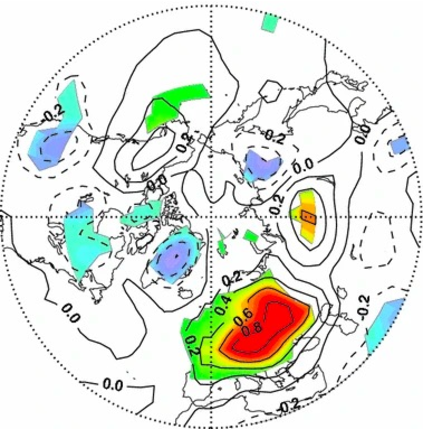
\includegraphics[scale=0.6]{master_thesis_contents/master_thesis_fig/rozanov2012_fig12.pdf}
        \label{fig:rozanov2012_fig12}
    \end{minipage}
    \begin{minipage}{\linewidth}
        \leftline{(b)}
        \centering
        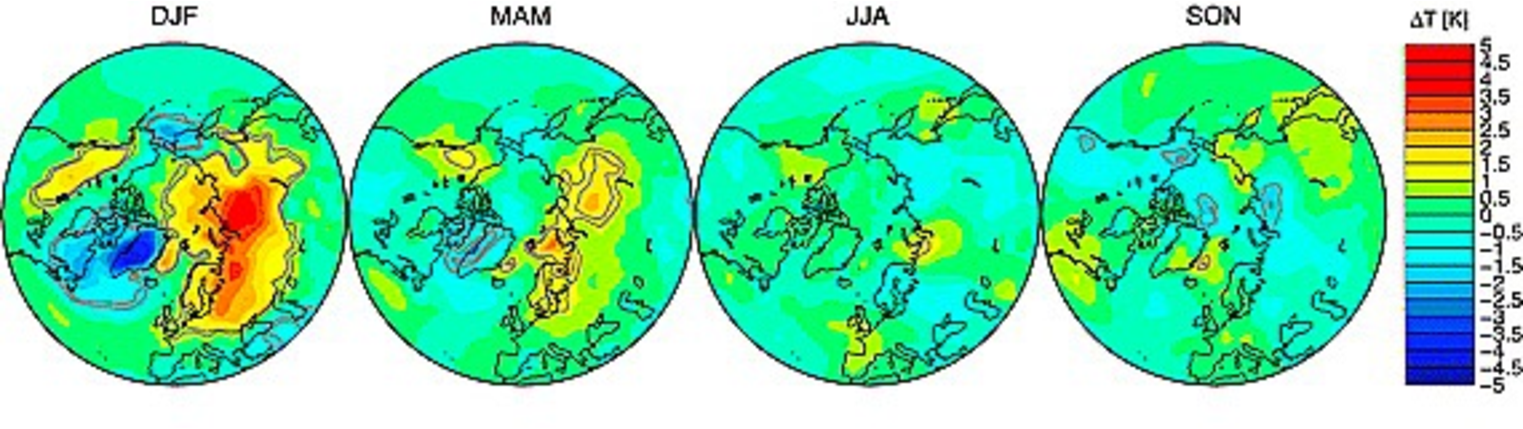
\includegraphics[scale=0.6]{master_thesis_contents/master_thesis_fig/seppala2009_fig3.pdf}
        \label{fig:seppala2009_fig3}
    \end{minipage}
    \caption{EPP時の地表温度の変化$\Delta T\, \mathrm{[K]}$。シュミレーション結果と観測結果の両方に地表温度の上昇が確認できるが、上昇のピークの値に差がある。(a)シミュレーション結果(最大で$0.8\, \mathrm{K}$の増加、~\cite{rozanov2012influence}より引用)(b)観測データに基づいた統計結果(最大で$5\, \mathrm{K}$の増加、~\cite{seppala2009geomagnetic}より引用)}
    \label{fig:rozanov2012_seppala2009}
\end{figure}
そこで我々の研究グループでは、EPPの影響による\ce{O3}の変動を観測的に明らかにすることを目的の1つとして研究を行っている。
EPPの影響による\ce{O3}の変動は、図~\ref{fig:epp_to_ozone_flow}のようなシナリオが考えられている~\cite{rozanov2012influence}。
\begin{figure}[htbp]
    \centering
    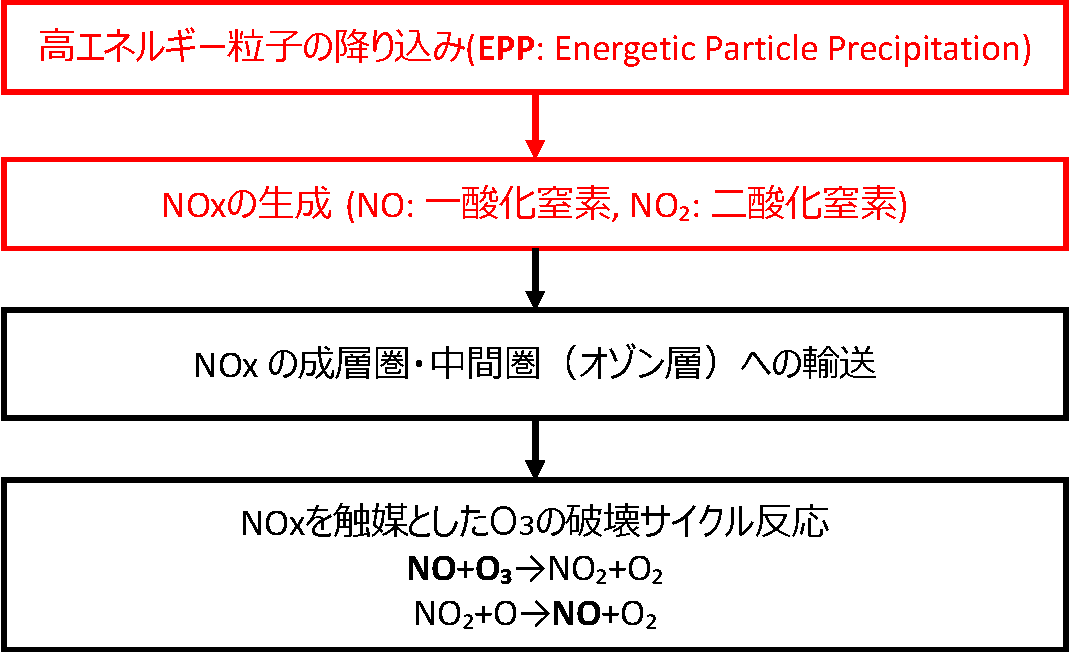
\includegraphics[width=\linewidth]{master_thesis_contents/master_thesis_fig/epp_to_ozone_flow.pdf}
    \caption{EPPから\ce{O3}破壊までのフロー}
    \label{fig:epp_to_ozone_flow}
\end{figure}
まずEPPが起きると、それによって上部中間圏〜熱圏の高度で$\mathrm{NO}_x$と呼ばれる一酸化窒素\ce{NO}や二酸化窒素\ce{NO2}が生成される。
それが大気の鉛直輸送によって成層圏・中間圏に輸送されることにより、図~\ref{fig:rozanov2012_seppala2009}の反応式で表されるように\ce{O3}の破壊サイクル反応を起こす。


\section{先行研究の結果と課題}
\label{sec:intro_privious}
先行研究ではEPPによって$\mathrm{NO}_x$が増加し、それが\ce{O3}の変動に影響を与えていることがMIPASによる衛星観測のデータにて時間分解能が1日ではあるが示されている(図~\ref{fig:lopez2005observation_fig3})~\cite{lopez2005observation}。
2003年10月28日にEPPがあったが、その後に$\mathrm{NO}_x$の増加が確認されており、$\mathrm{NO}_x$の増加があった領域において\ce{O3}の減少が確認できる。
\begin{figure}[htbp]
    \centering
    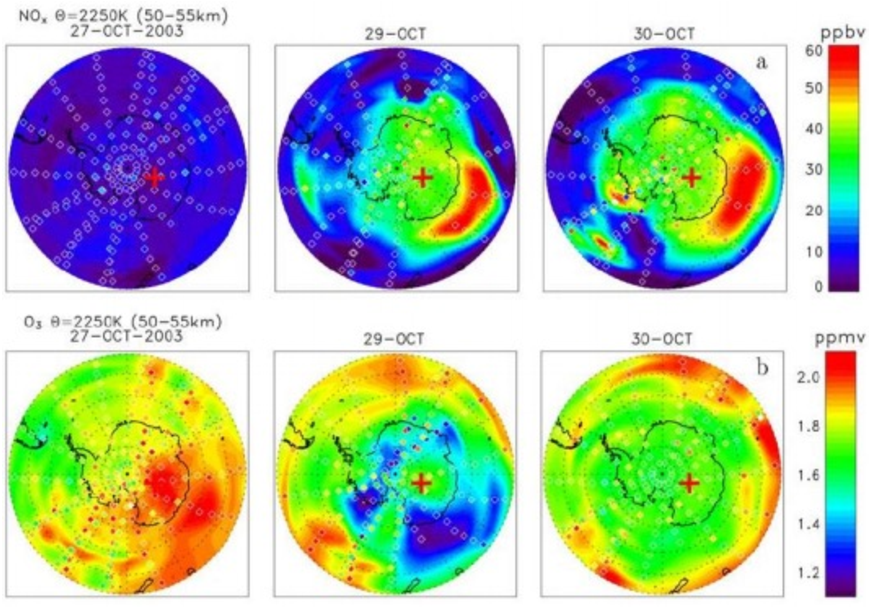
\includegraphics[width=\linewidth]{master_thesis_contents/master_thesis_fig/lopez2005observation_fig3.pdf}
    \caption{EPPイベントの前後での南半球の高度$50-55\, \mathrm{km}$における$\mathrm{NO}_x$と\ce{O3}の変動(~\cite{lopez2005observation}より引用)}
    \label{fig:lopez2005observation_fig3}
\end{figure}
MIPASは太陽同期軌道を周回する衛星であり、リム観測で大気分子観測を行う衛星である。
このような衛星観測はこの図で示されるように全球的な観測を行うことには向いているが、衛星軌道の特性により時間分解能は1日と比較的悪く、ある一地点における高時間分解能かつ連続的な観測には向いていないという課題があった。
その課題を克服するため、我々の研究グループではミリ波分光計(観測手法の詳細は\ref{ch:mm_obs}章で述べる)を用いた観測を行っている。\par
ミリ波分光を用いた地上観測と衛星観測は相補的な関係にあるため、必要に応じて衛星観測のデータを補足的に用いる。
% 修正済
% どちらが優れているとか、ミリ波観測があれば衛星観測は不要、という主張に受け取られないように、それらの観測は相補的であるという文章があると良い。
次に、我々の研究グループが行ったミリ波分光計を用いたこれまでの研究について紹介する。
我々は、2011年から南極昭和基地でミリ波分光計による\ce{O3}と\ce{NO}の地上観測を行っている。
図~\ref{fig:isono2014ground_fig5a}は、2012年から2013年までの観測による\ce{NO}の柱密度の時間変動の結果である~\cite{isono2014ground}。
横軸が時系列になっていて、エラーバー付きのプロットは\ce{NO}の柱密度を示しており1日1プロットである。
背景の紫色の影の部分は、高度$100\, \mathrm{km}$におけるそれぞれの日で太陽が当たっていない時間の長さを表している。
この結果より、季節変化にともなう長期的な変動のほか、冬期(4月〜8月頃)には4日程度の顕著な短期的変動が確認できた。
この短期的な変動は、EPPにともなう現象であると考えられる。
しかし一方で、\ce{NO}は光解離するため、夏(10月〜翌年2月頃)においては太陽光による影響も考慮に入れる必要がある。
そのため、夏においてはEPPイベントの際に、\ce{NO}の増加と、光解離による\ce{NO}の減少が同時に起きるため、光解離の影響とEPPの影響は切り分けることができなかった(図~\ref{fig:isono2014ground_fig5a}の紫色の影の部分がない時期のプロット。エラーバーの範囲を超えた顕著な短期変動は確認できない)。
\begin{figure}[htbp]
    \centering
    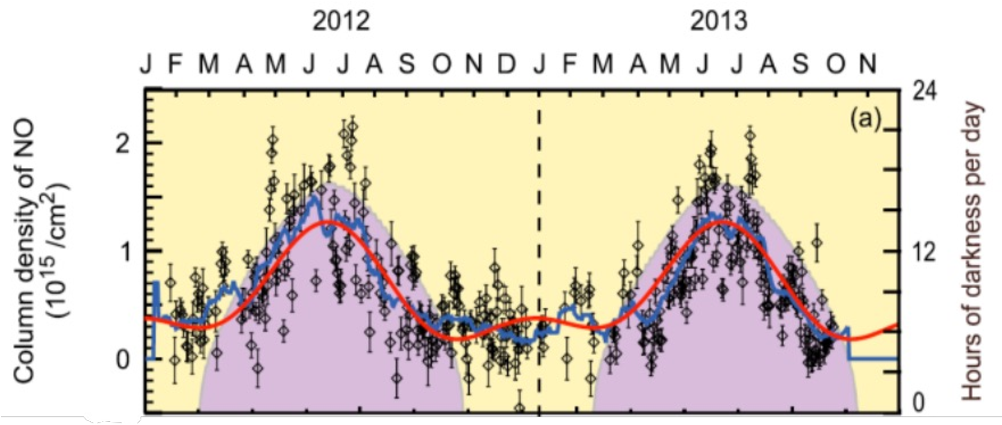
\includegraphics[width=\linewidth]{master_thesis_contents/master_thesis_fig/isono2014ground_fig5a.pdf}
    \caption{ミリ波分光計を用いた観測による南極・昭和基地での\ce{NO}の変動(エラーバー付きのプロットは\ce{NO}の柱密度を示しており1日1プロットである。
    紫色の影の部分は、高度$100\, \mathrm{km}$におけるそれぞれの日で太陽が当たっていない時間を表している。青色の線は31日間の移動平均、赤色の線は年周期成分と半年周期成分からなる正弦波によるフィッティングを行ったもの。~\cite{isono2014ground}より引用)}
    \label{fig:isono2014ground_fig5a}
\end{figure}
以上のことを踏まえて、先行研究での衛星観測とミリ波分光計での地上観測で明らかになったことと、それらの課題点についてまとめる。
\clearpage
\begin{itemize}
    \item 明らかになった点
    \begin{itemize}
        \item ミリ波分光を用いた地上観測(南極・昭和基地)
        \begin{itemize}
            \item 季節にともなう\ce{NO}の長期的変動
            \item EPPに伴う\ce{NO}の増加
        \end{itemize}
        \item 衛星観測
        \begin{itemize}
            \item EPPに伴う高度$50\, \mathrm{km}$付近のグローバルな\ce{NO}の増加
            \item \ce{NO}の増加した領域での\ce{O3}の減少
        \end{itemize}
    \end{itemize}
    \item 課題点
    \begin{itemize}
        \item ミリ波分光計を用いた地上観測(南極・昭和基地)
        \begin{itemize}
            \item 夏の\ce{NO}の短期変動の確認が難しい
        \end{itemize}
        \item 衛星観測
        \begin{itemize}
            \item 定点での連続的な観測が難しい
        \end{itemize}
    \end{itemize}
\end{itemize}
\ref{sec:intro_porpose}節では、これらの課題点を踏まえた本研究の目的について述べていく。


\section{本研究の目的と研究手法}
\label{sec:intro_porpose}
本研究では、図~\ref{fig:epp_to_ozone_flow}で示したEPPによる\ce{O3}破壊現象のフローの中で、まずは上の2つの関係の解明に取り組んだ(図~\ref{fig:flow_and_porpose}中の赤枠)。
EPPについては、Dst指数と呼ばれる地磁気擾乱の大きさを表す指数と衛星観測による電子フラックスデータから現象の同定を行い、その規模などの特性を調べた。
加えて、NASAが提供しているOMNI Data Setを用いて、電子フラックスの増加の原因となる事象が何かを調べた。
$\mathrm{NO}_x$については、ミリ波観測による\ce{NO}のスペクトルデータから柱密度を導出し、その時間変動について調べた。
最後に、これらの関係性について調べることにより、EPPがどのように\ce{NO}の変動に影響を与えているかについて明らかにする。
\begin{figure}[htbp]
    \centering
    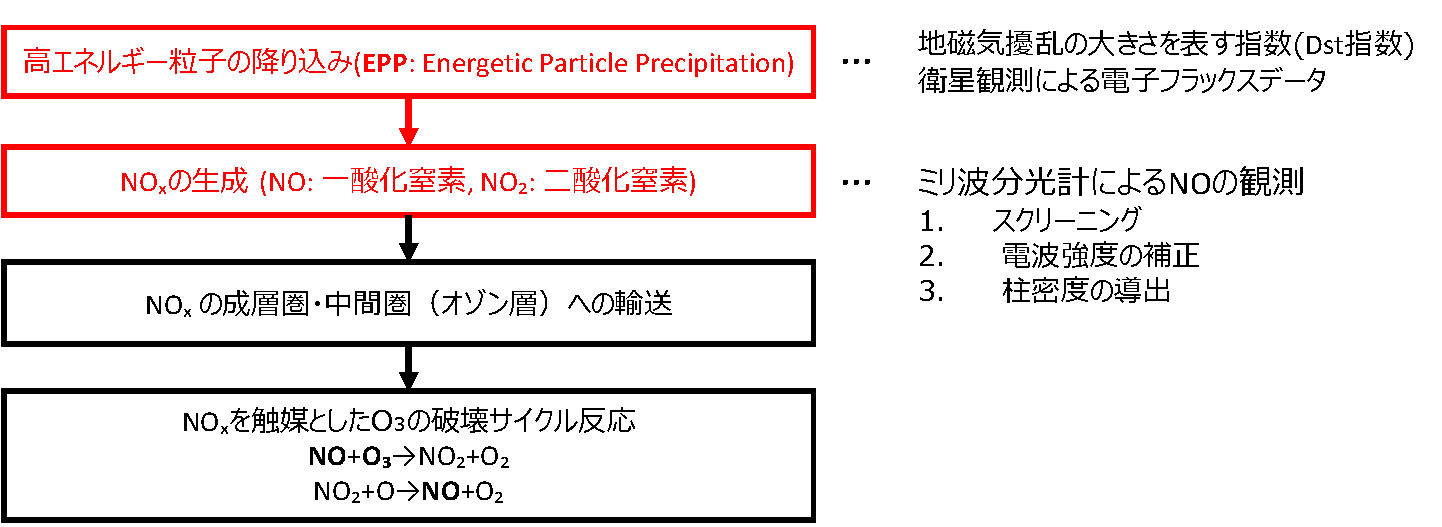
\includegraphics[width=\linewidth]{master_thesis_contents/master_thesis_fig/flow_and_porpose.pdf}
    \caption{EPPによる\ce{O3}破壊現象の流れと本研究の目的・手法との対応}
    \label{fig:flow_and_porpose}
\end{figure}


% \chapter{ミリ波観測手法}
\chapter{ミリ波観測法}
\label{ch:mm_obs}

\ref{ch:mm_obs}章では、我々が開発したミリ波分光計を用いた大気分子の観測手法について述べる。
まず\ref{sec:mm_obs}節では観測手法の概観を紹介し、観測された電波強度のキャリブレーション方法、受信電波から分子スペクトルを抽出するために行う周波数スイッチング、下層大気の影響を評価し除去するための光学的厚みの測定について述べる。
次に、本研究で使用したミリ波分光計について、\ref{subsec:mm_tromsoe}節でノルウェーのトロムソに設置した装置、\ref{subsec:mm_syowa}節で南極の昭和基地に設置された装置についてそれぞれ説明する。


\section{観測手法}
\label{sec:mm_obs}
\subsection{観測手法の概観と観測装置}
最初に、ミリ波分光法を用いた大気分子の観測手法について述べる。
私たちのグループでは、観測の手法としてミリ波電波分光法による地上観測によって大気分子を観測している~\cite{mizuno2002millimeter}。
その模式図を図\ref{fig:spectrometer_schema}に示す。
\begin{figure}[htbp]
    \centering
    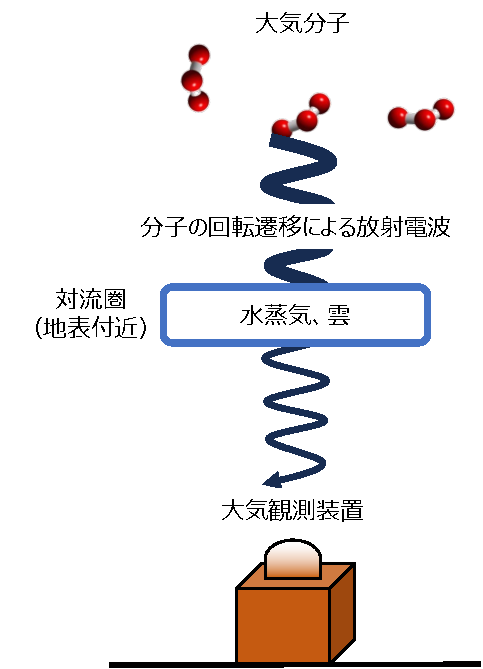
\includegraphics{master_thesis_contents/master_thesis_fig/spectrometer_schema.pdf}
    \caption{ミリ波電波分光法による地上観測の模式図}
    \label{fig:spectrometer_schema}
\end{figure}
% 「下層大気」
% この場合、「下層大気」とは何でしょうか?高度軸は、対流圏・成層圏などの言葉を使い(もしくは高度を数字で書いても良い)、もう少し正確・定量的に描いた方が良い。

ミリ波電波分光法では、観測対象の大気分子の回転遷移によって放射されるミリ波帯電波を受信し分光することで、電波放射スペクトルを観測している。
しかし、図\ref{fig:spectrometer_schema}に示す通り、電波を地上で観測すると、経路上にある下層大気の水蒸気や雲の影響を考慮する必要があることに注意しなければならない。
この影響は、下層大気の光学的厚みを実際に計測することで、補正ができる。
光学的厚みの測定方法の詳細は\ref{subsec:opticaldepth}節にて述べる。\par

ミリ波分光計を用いた大気観測装置の構成を図\ref{fig:mm_component}に示し、例として南極の昭和基地に設置された大気観測装置の様子を図\ref{fig:mmobs_spectrometer_syowa}に示す。
図\ref{fig:mm_component}に示すように、観測装置は主に以下の4つの部分に分かれている。
\begin{figure}[htbp]
    \centering
    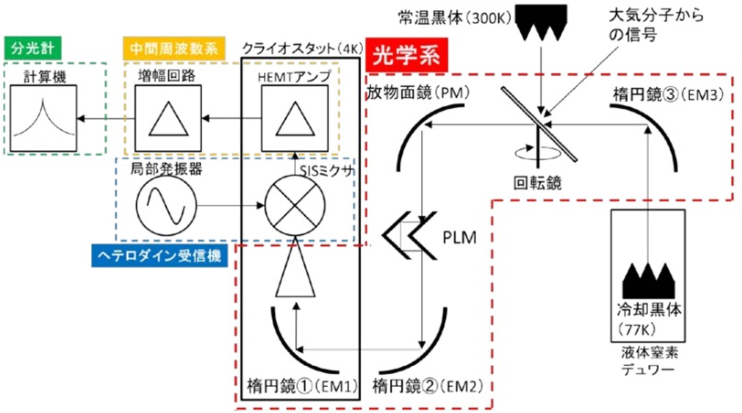
\includegraphics[width=\linewidth]{master_thesis_contents/master_thesis_fig/mm_component.pdf}
    \caption{ミリ波大気観測装置の概略図(~\cite{ito2017master}より引用)}
    % \caption{$\scriptstyle \mbox{ミリ波大気観測装置の概略図}\atop \scriptstyle \mbox{text}(~\cite{ito2017master}より引用$}
    \label{fig:mm_component}
\end{figure}
\begin{figure}[htbp]
    \centering
    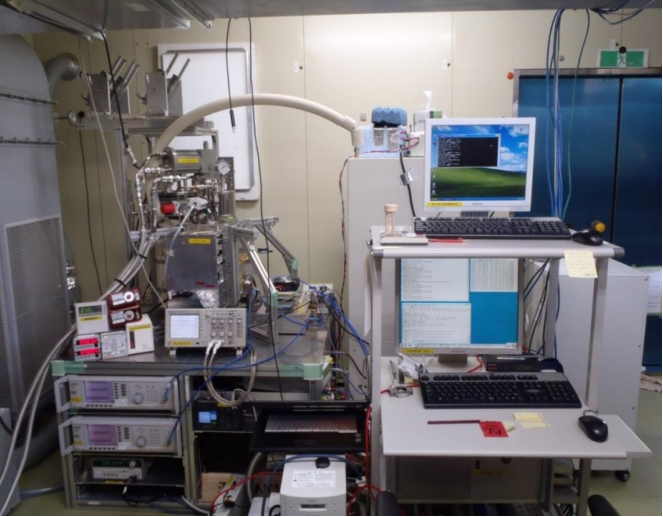
\includegraphics[width=\linewidth]{master_thesis_contents/master_thesis_fig/mmobs_spectrometer_syowa.pdf}
    \caption{南極の昭和基地に設置された観測装置(~\cite{uemura2014master}より引用)}
    \label{fig:mmobs_spectrometer_syowa}
\end{figure}
\begin{enumerate}
    \item 光学系 \par
        大気分子からの信号を集光し伝送するための複数の鏡と電磁ホーンによって構成される。
        また、回転鏡を用いることにより、強度キャリブレーションに用いる基準雑音信号として、常温黒体($300\, \mathrm{K}$)と冷却黒体($77\, \mathrm{K}$)からの放射も入力できるようになっている。
        大気分子からの信号とその信号のキャリブレーション(詳細は\ref{subsec:calibration}節)で用いる常温黒体と冷却黒体の測定との切り替えを行う。
        PLM(光路長変調器: Path Length Modulator)は光学系にて発生する定常波を除去する役割がある。
    \item ヘテロダイン受信機 \par
        大気分子からの信号を局部発振器からの信号とSISミクサで混合する。
        大気分子からの電波は微弱であるため、信号処理に適切なレベルまで増幅しなければならない。
        しかし、本研究で扱う電波の周波数(数百GHz程度)を直接増幅できる増幅器は、現在のところ実用レベルでは存在しない。
        そこで、受信した信号をSISミクサを用いて低い周波数(数GHz程度)に下げることにより、一般的なマイクロ波帯のHEMTアンプによって増幅する方法をとっている。
        このような受信方法をヘテロダイン方式と呼ぶ。
    \item 中間周波数系 \par
        ミクサから出力された信号を後段の分光計にとって適切な周波数にさらに変換し、必要な電波強度レベルまで増幅する。
    \item 分光計 \par
        入力信号を直接A/D変換して時系列データとして読み込み、それを高速フーリエ変換することにより大気分子の周波数スペクトルを得る。
        本研究で用いた大気分子のスペクトルデータを得るために使用された分光計は
        % 追加:「、**社の**であり、その仕様としては」
        16348チャンネルの周波数スペクトルデータを出力する~\cite{ito2017master}。
        % 昭和基地の場合のチャンネル数は?引用元をみないといけない
        % もし分光計の仕様を紹介したいのであれば、チャネル数だけを書くというのはあまり意味がありません。たとえば、大山さんの論文を見て、分光計の諸元として何が書かれているかを参考にすると良い。
\end{enumerate} \par
ミリ波電波分光法による地上観測による最大の利点は、太陽光などの背景光源を必要としないため、昼夜を問わず連続的なモニタリングが可能なことである。
これは、昼夜だけでなく白夜や極夜がある極地においても、その影響を受けずに連続観測することができる唯一の手法であることを意味している。
以上より、連続的・長期的に観測を行うことが可能で、一地点において観測することにより自然起源や人為起源による長期的変動や短期的変動を観測することが可能であり、これが我々の研究グループがミリ波電波分光法による地上観測という世界的に見てもユニークな手法に力を入れている理由である。

\subsection{電波強度のキャリブレーション}
\label{subsec:calibration}
次に、観測された電波に対して黒体を用いて行う強度キャリブレーションの手法について述べる。
一般的に電波領域の研究では、大気分子からの電波放射強度は、それと同等のエネルギーを放射する黒体の温度に換算して表す。ここでミリ波領域(周波数$30-300\, \mathrm{GHz}$)においては、図\ref{fig:planck}よりRayleigh-Jeans近似が成り立つので、ほぼPlanckの放射式は以下のように表すことができる。
\begin{gather}
    I_{\nu}(T)
    = \frac{2\mathrm{h}\nu^3}{c^2} \cdot \cfrac{1}{\exp \Biggl( \cfrac{\mathrm{h}\nu}{\mathrm{k}T}-1\Biggr) }
    \approx \frac{2\mathrm{h}\nu^3}{c^2} \cdot \left(\frac{\mathrm{h}\nu}{\mathrm{k}T}\right)^{-1}
    = \frac{2\nu^2}{c^2}\mathrm{k}T \\
    I_\nu(T):電波強度、c:光速、\mathrm{k}:Boltzmann定数、\mathrm{h}:Planck定数、\nu:周波数、T:黒体温度 \notag
    \label{eq:planck}
\end{gather}
\begin{figure}[htbp]
    \centering
    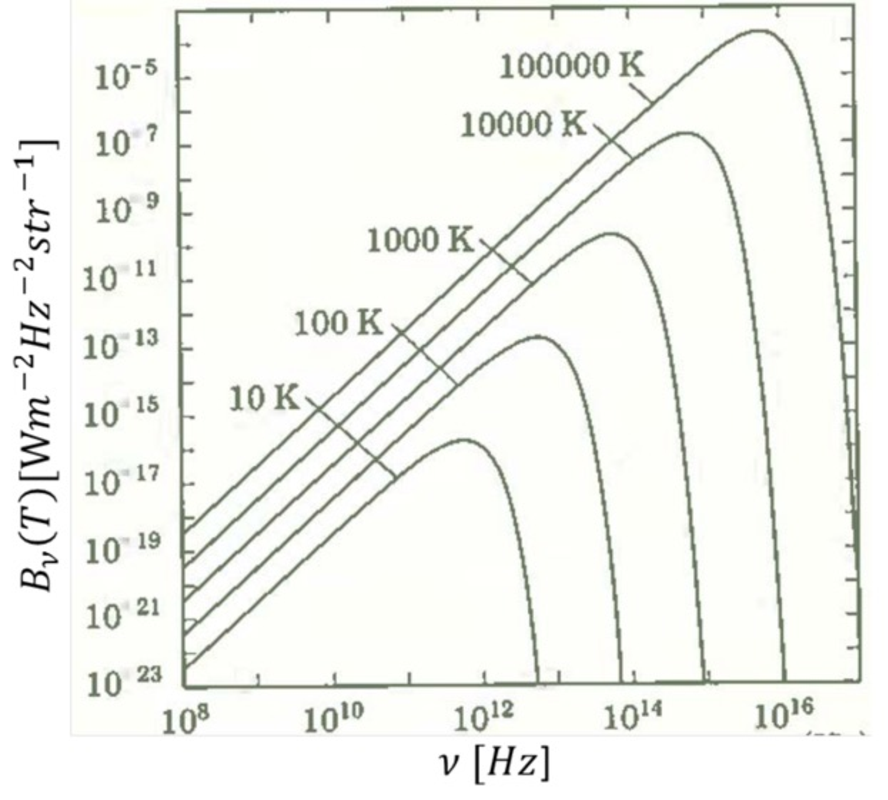
\includegraphics[width=\linewidth]{master_thesis_contents/master_thesis_fig/planck.pdf}
    \caption{Planckの放射式(~\cite{ito2017master}より引用)}
    \label{fig:planck}
\end{figure}
この式から黒体温度と電波強度は比例の関係になるため、大気分子からの電波強度を黒体の温度に換算することが可能である。
具体的には常温黒体(多くの場合室温の$300\ \mathrm{K}$)と液体窒素で冷却された黒体($77\ \mathrm{K}$)からの電波放射を受信機に入れることにより、受信電波強度を黒体の温度スケーリングする(これを強度較正あるいは強度キャリブレーションと呼ぶ)。
\begin{figure}[htbp]
    \centering
    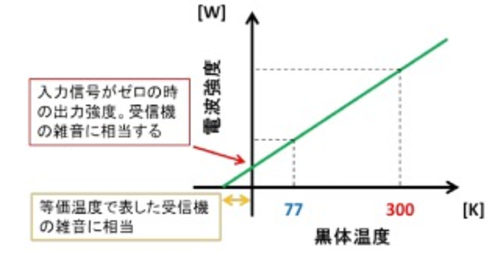
\includegraphics[scale=0.6]{master_thesis_contents/master_thesis_fig/calibration.pdf}
    \caption{電波強度のキャリブレーションの様子(~\cite{ito2017master}より引用)}
    \label{fig:calibration}
\end{figure}
これを図示すると、図\ref{fig:calibration}に示す直線が電波強度と黒体温度の対応を表す。
また、この直線の$y$切片の値は受信機雑音の強度を表し、$x$切片の値の絶対値はこの強度を黒体温度で表した値となる。

\subsection{光学的厚み}
\label{subsec:opticaldepth}
次に、受信された電波強度について、下層大気の影響の補正に用いる光学的厚みについて述べる。
図\ref{fig:spectrometer_schema}に示したように、成層圏よりも高い高度にある分子からの電波を地上で観測する際には、下層大気(主に対流圏)を通過してきた電波を観測することになる。
そのため、下層大気に含まれる水蒸気や雲の放射および吸収の影響を考慮に入れる必要があり、光学的厚みという概念を導入する。\par

まず、光学的厚みとは何かということと、それがどのように電波強度に影響するかを述べる。
図\ref{fig:depth_dx}のように、厚さ$dx$の大気層があり、図の左から強度$T$の電波が入射したときを考える。
大気層で吸収および放射の影響を受けて、図の右に出てくる電波強度は$T+dT$で表される。
\begin{figure}[htbp]
    \centering
    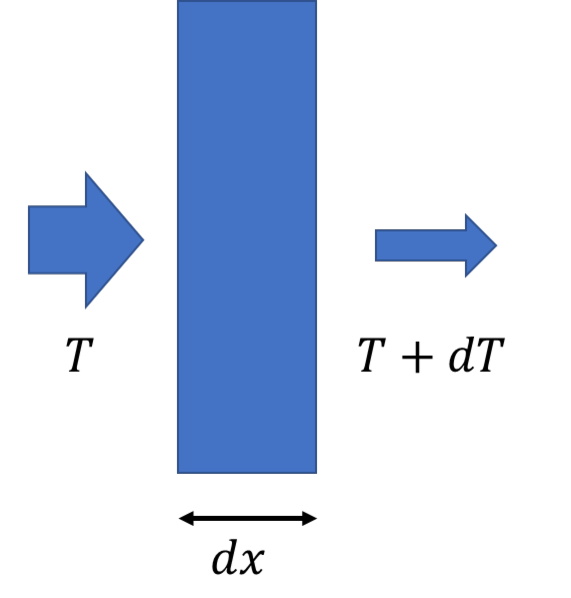
\includegraphics{master_thesis_contents/master_thesis_fig/depth_dx.pdf}
    \caption{厚さ$dx$の大気層を通過する電波強度の模式図}
    \label{fig:depth_dx}
\end{figure}
このとき、吸収と自己放射を表す式は、$\kappa$を吸収係数、$j$を放射係数とすると
\begin{equation}
    dT = -\kappa T dx + j dx
    \label{eq:absorption_selfemission_1}
\end{equation}
となる。
次に光学的厚み(一般的に$\tau$で表す)を導入する。$\tau$は、
\begin{equation}
    \tau = \int_{0}^{x} \kappa dx' + j dx
\end{equation}
もしくは
\begin{equation}
    d\tau = \kappa dx
\end{equation}
と表され、これを用いて式\eqref{eq:absorption_selfemission_1}を書き換えると
\begin{equation}
    \frac{dT}{d\tau} = -T + \frac{j}{\kappa}
    \label{eq:absorption_selfemission_4}
\end{equation}
となる。
次に、式\eqref{eq:absorption_selfemission_4}の第2項において、熱平衡状態ではキルヒホッフの法則より
\begin{gather}
    \frac{j}{\kappa}
    = \frac{2\mathrm{h}\nu^3}{c^2} \cdot \cfrac{1}{\exp\Biggl(\cfrac{\mathrm{h}\nu}{\mathrm{k}T}-1\Biggr)}
    \equiv I_\nu
    = T_\mathrm{sky}
    \label{eq:absorption_selfemission_5} \\
    % I_\nu :電波強度、T_{sky}:大気からの熱放射、c:光速、k:Boltzmann定数 \notag \\
    % h:Planck定数、\nu :周波数、T:黒体温度 \notag
    T_\mathrm{sky}:大気からの熱放射 \notag
\end{gather}
が成り立つ。
これを利用して式\eqref{eq:absorption_selfemission_5}より式\eqref{eq:absorption_selfemission_4}の解を求めると、
\begin{gather}
    T = T_0\exp\left(-\tau\right) + T_\mathrm{sky}\left(1-\exp\left(-\tau\right)\right) + T_\mathrm{sys}
    \label{eq:absorption_selfemission_6} \\
    T_0 :大気分子からの電波強度、T_\mathrm{sky}:受信機雑音 \notag
\end{gather}
となる。
これは、第1項が下層大気による電波吸収を考慮した(より上層にある)観測対象の分子からの電波強度、第2項は下層大気の熱放射を表している。
実際の観測で得られるスペクトルデータとしては第1項が図\ref{fig:spectum_thermalnoise}における橙色の成分、第2項が青色の成分に対応する(実際には青色の成分に第3項の受信機雑音も含まれるが、その詳細は\ref{subsec:frsw}節にて述べる)。
\begin{figure}[htbp]
    \centering
    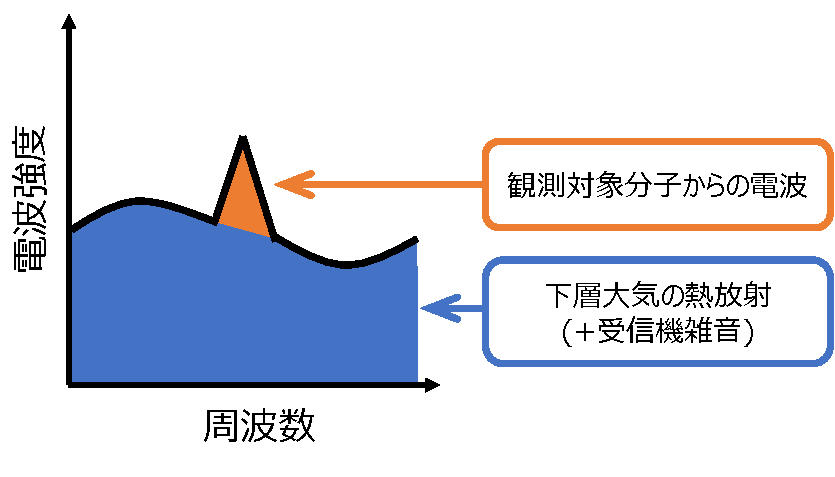
\includegraphics[width=\linewidth]{master_thesis_contents/master_thesis_fig/spectum_thermalnoise.pdf}
    \caption{スペクトルデータの強度を決める要素}
    \label{fig:spectum_thermalnoise}
\end{figure}
式\eqref{eq:absorption_selfemission_6}の左辺$T$が観測値として直接的に得られる電波強度であるが、我々が知りたい値は、もともとの放射強度である$T_0$であるので、$T_0$を知るためには光学的厚みの補正が必要となるわけである。\par

次に、光学的厚みをどのように測定するかについて述べる。
光学的厚みの測定は図\ref{fig:opticaldepth_measurement}のように観測の間に定期的に行われており、たとえばトロムソの観測装置ではおよそ5分おきに測定されている。
% 昭和基地も同じなのか?
\begin{figure}[htbp]
    \centering
    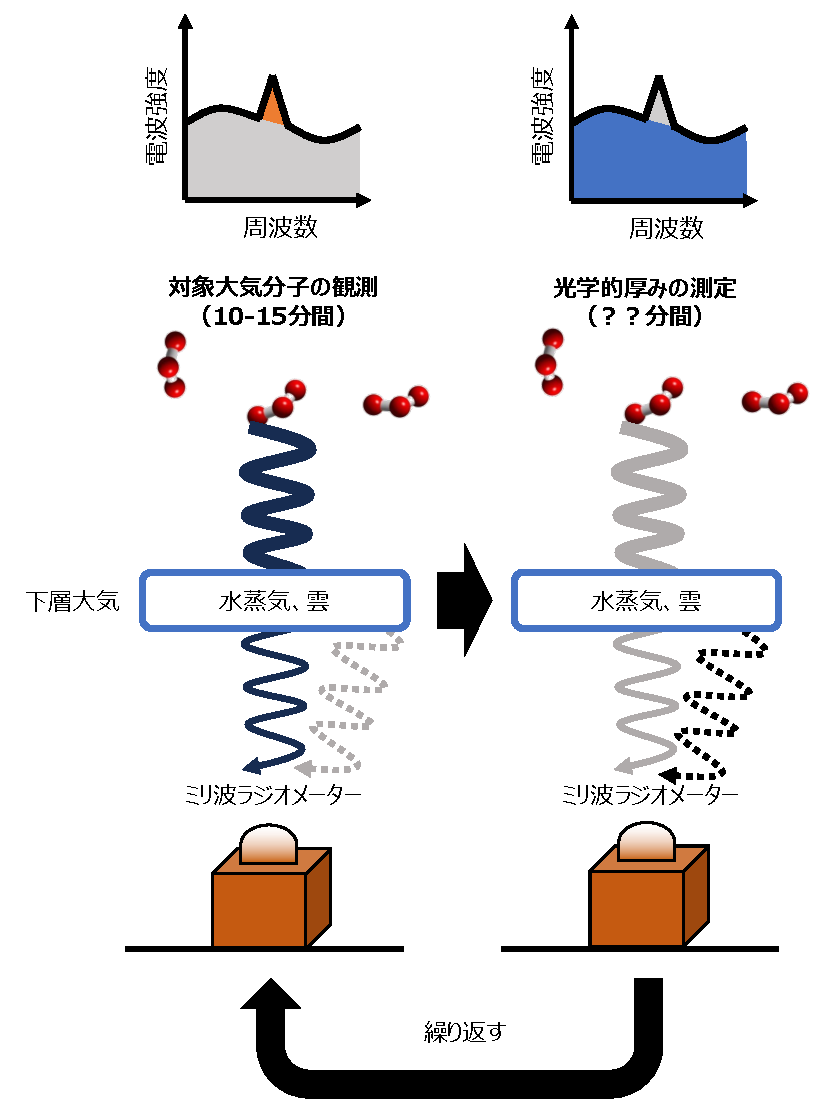
\includegraphics[width=\linewidth]{master_thesis_contents/master_thesis_fig/opticaldepth_measurement.pdf}
    \caption{ミリ波観測と光学的厚み$(\tau)$の測定の流れ}
    \label{fig:opticaldepth_measurement}
\end{figure}
% この図は必要でしょうか?図が無いと理解できないほどの内容ではないのと、図が何を説明したいのか、良く分かりませんでした。
測定された光学的厚みの値は、直前に観測された電波強度のデータの補正に用いられる。
光学的厚みの測定についてはSky tippingと呼ばれる手法が用いられる。
% Sky tippingの文献がありませんか。
まず関係式として、以下の二式を用いる。
\begin{gather}
    \begin{cases}
        T_z = T_\mathrm{sky} \left\{ 1-\exp \left(-\tau \sec z \right)  \right\} + T_\mathrm{sys} \\
        T_\mathrm{obs\_ hot} = T_\mathrm{hot} + T_\mathrm{sys}
    \end{cases}
    \label{eq:opticaldepth_measurement} \\ \notag
    z :観測する角度の天頂角 \\ \notag
    T_\mathrm{z} :天頂角zでの分子スペクトルを含まない周波数の信号強度 \\ \notag
    % T_{sky} :大気からの熱放射、T_{sys} :観測装置の自己雑音温度 \\ \notag
    T_\mathrm{obs\_ hot} :常温黒体を見たときの輝度温度 \\ \notag
\end{gather}
ここで、$T_\mathrm{sky} = T_\mathrm{hot}$と仮定し式\eqref{eq:opticaldepth_measurement}の2式の差をとって両辺対数をとると
\begin{equation}
    \ln \left( T_{obs\_ hot} - T_z \right)  = \ln T_{obs\_ hot} - \tau \sec z
    % \ln \( T_{obs\_ hot} - T_z \) = \ln T_{obs\_ hot} - \tau \sec z
\end{equation}
となる。
この式は$y=ax$のような一次関数になっているため、左辺$\ln \left( T_\mathrm{obs\_ hot} - T_z \right)$を縦軸、$\sec z$を横軸としたプロットを作成すると、図\ref{fig:opticaldepth_slope_tau}のようになることがわかる(プロットデータは観測装置の回転鏡により$z$の値を変えている)。
これらのプロットに対して一次の近似直線を引いたとき、その直線の傾きが光学的厚みに負の符号をつけたものと対応する。
以上より、光学的厚みを観測的に求めることができる。\par

\begin{figure}[htbp]
    \centering
    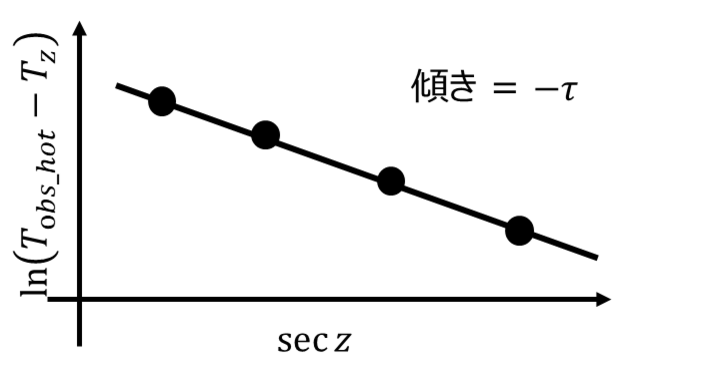
\includegraphics[width=\linewidth]{master_thesis_contents/master_thesis_fig/opticaldepth_slope_tau.pdf}
    \caption{光学的厚み$\tau$を求めるためのプロットデータの模式図}
    \label{fig:opticaldepth_slope_tau}
\end{figure}
トロムソの観測装置で実際に測定している$\sec z$の値は、表\ref{tb:secz_zdeg}のようになっている。
ここでは、それに対応した天頂角$z$と仰角の値も示す。
\begin{table}[htbp]
    \centering
    \caption{$\sec z$と天頂角$z\ [ \deg ]$と仰角$[ \deg ]$との対応}
    \label{tb:secz_zdeg}
    \setlength{\belowcaptionskip}{5mm}
    \begin{tabular}{ccc}
    \hline
    $\sec z$ & 天頂角 $z\ [ \deg ]$ & 仰角$[ \deg ]$ \\ \hline
    1.46 & 47 & 43 \\ \hline
    1.83 & 57 & 33 \\ \hline
    2.28 & 64 & 26 \\ \hline
    2.79 & 69 & 21 \\ \hline
    \end{tabular}
\end{table}


\subsection{周波数スイッチング}
\label{subsec:frsw}
観測されたスペクトルデータから対象の分子スペクトルのみを得るためには、大気の熱放射と観測装置の受信機雑音によるオフセット成分を除去する必要がある。
このオフセットを除去するにはいくつかの手法が行われているが、本研究で使用する観測装置では、周波数スイッチング(以後FRSWとする)という手法を用いる。
% (図\ref{fig:frsw_schema})
% \begin{figure}[htbp]
%     \centering
%     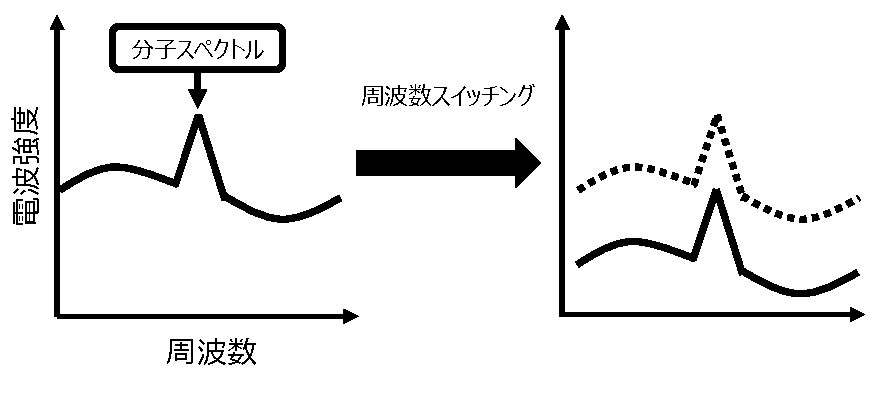
\includegraphics[width=\linewidth]{master_thesis_contents/master_thesis_fig/frsw_schema.pdf}
%     \caption{周波数スイッチング(FRSW)の模式図}
%     \label{fig:frsw_schema}
% \end{figure}
% 図は必要なしか。
ただし、FRSWによるオフセット成分の除去はおおまかなものであるため、本研究のように弱いスペクトルを検出する必要がある場合には、さらに細かくオフセット成分を補正する処理が必要となる(詳細は\ref{sec:correction_baselinefitting}節で述べる)。
本研究では、ハードウェアでのFRSWによるデータ取得に加えて、周波数折返し処理という解析方法を用いる。
この手法を用いることで、オフセット成分を除去するとともに、スペクトルデータの信号対雑音比(S/N比)を向上させている。\par

\begin{figure}[htbp]
    \centering
    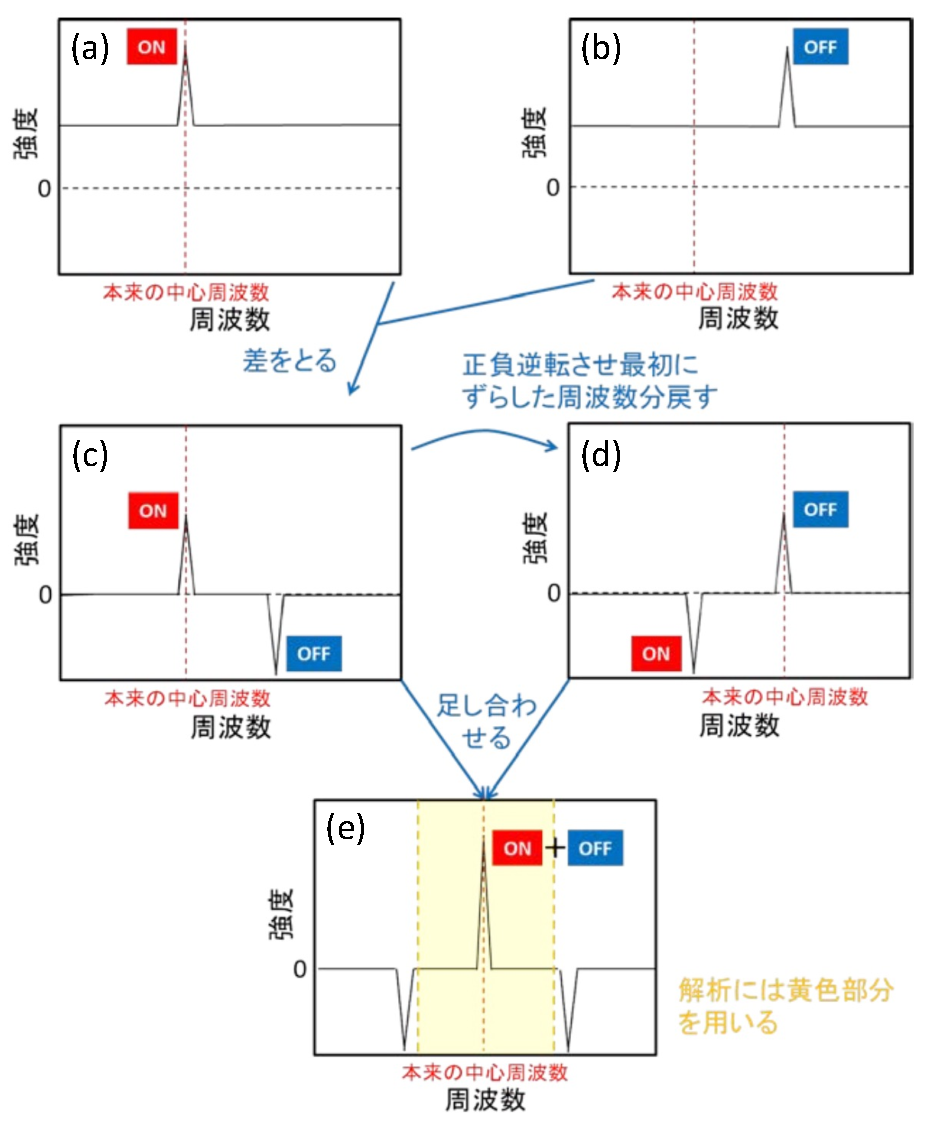
\includegraphics[width=\linewidth]{master_thesis_contents/master_thesis_fig/frsw_process.pdf}
    \caption{周波数スイッチングと周波数折り返し処理の概要(\cite{ito2017master}より引用)}
    \label{fig:frsw_process}
\end{figure}
まず、ハードウェア的に行われるFRSWについて説明する。
ある周波数において最初に取得されるデータを図\ref{fig:frsw_process}(a)に示す。
次に、局部発振器の周波数を$\Delta f$ずらした状態でデータを取得する(図\ref{fig:frsw_process}(b))。
これにより、分光計のチャンネル上では、異なるチャンネルに同じ分子からの輝線スペクトルが現れる2つのデータが得られる。
その次に、解析では、まず(a)から(b)を差し引いたデータを作成する(図\ref{fig:frsw_process}(c))。
これにより、(a)と(b)に共通に乗っていたオフセット成分が差し引かれる。
さらに(c)を上下反転して、ずらした周波数$\Delta f$を戻した(d)を作成する。
この(d)と(c)のデータを足し合わせて2で割る処理をする(周波数折り返し処理)。
(a)と(b)で取得された輝線スペクトルのデータは独立なものなので、この処理をすることによって、大気雑音や受信機雑音などのランダムなノイズ成分が低減し、S/N比としては$\sqrt{2}$倍向上する(図\ref{fig:frsw_process}(e))。
そして、最終的に得られる分子スペクトルとしては、図\ref{fig:frsw_process}(e)中の黄色で囲まれたところのみを使う。
\clearpage


\section{観測場所}
\label{sec:obs_location}
\ref{sec:obs_location}節では、解析に用いたノルウェーのトロムソと南極の昭和基地のミリ波分光計について、それぞれ観測を立ち上げた時期と設置されてきた分光計の概要を述べる。トロムソと昭和基地で設置された分光計の仕様を表\ref{tb:spectrometer_spec}に示す。
\begin{table}[htbp]
    \centering
    \caption{トロムソ(1段目)と昭和基地(2段目)で設置された分光計の仕様}
    \label{tb:spectrometer_spec}
    \setlength{\belowcaptionskip}{5mm}
    \resizebox{\columnwidth}{!}{%
    \begin{tabular}{ccccc}
    \hline
    &
        期間 &
        FrontEnd &
        BackEnd &
        観測対象の分子 \\ \hline
    単周波数分光計 &
        2016年 - &
        \begin{tabular}[c]{@{}c@{}} Double sideband\\ PCTJ  SIS mixer\end{tabular} &
        \begin{tabular}[c]{@{}c@{}}FFT 分光計\\ 帯域 $\sim1\ \mathrm{GHz}$\\ 分解能 $\sim61\ \mathrm{kHz}$\end{tabular} &
        \begin{tabular}[c]{@{}c@{}}\ce{NO}, \ce{O3} \\ (切替観測)\end{tabular} \\ \hline
    % Multi-freq. Phase 1 &
    %     \begin{tabular}[c]{@{}c@{}}2020年11月 – \\ 2021年2月\end{tabular} &
    %     \begin{tabular}[c]{@{}c@{}}2 Single sideband\\ PCTJ SIS mixers\end{tabular} &
    %     \begin{tabular}[c]{@{}c@{}}FFT 分光計\\ 帯域 $\sim$1GHz\\ 分解能 $\sim$61 kHz\end{tabular} &
    %     \begin{tabular}[c]{@{}c@{}}\ce{NO}, \ce{O3}, \ce{CO}, \ce{HO2} \\ (分子同時観測可能)\end{tabular} \\ \hline
    % Multi-freq. Phase 2 &
    %     \begin{tabular}[c]{@{}c@{}}2021年3月 –\\ 2022年1月\end{tabular} &
    %     \begin{tabular}[c]{@{}c@{}}1 Single sideband\\ PCTJ SIS mixers\end{tabular} &
    %     \begin{tabular}[c]{@{}c@{}}FFT 分光計\\ 帯域 $\sim$2 GHz\\ 分解能 $\sim$61 kHz\end{tabular} &
    %     \begin{tabular}[c]{@{}c@{}}\ce{NO}, \ce{O3}, \ce{HO2} \\ (分子同時観測可能)\\ (due to oscillator damage)\end{tabular} \\ \hline
    多周波数分光計 &
    % 多周波数分光計 Phase 3 &
        2022年7月 - &
        \begin{tabular}[c]{@{}c@{}}2 Single sideband\\ series-array SIS mixers\end{tabular} &
        \begin{tabular}[c]{@{}c@{}}FFT 分光計\\ 帯域 $\sim2.5\ \mathrm{GHz}$\\ 分解能 $\sim76\ \mathrm{kHz}$\end{tabular} &
        \begin{tabular}[c]{@{}c@{}}\ce{NO}, \ce{O3}, \ce{CO}, \ce{NO2}, \ce{HO2}\\ (同時観測)\end{tabular} \\ \hline
    \end{tabular}
    }
\end{table}

\subsection{ノルウェー・トロムソでの観測(69.35\textdegree N, 19.14\textdegree E)}
\label{subsec:mm_tromsoe}
\ref{sec:intro_privious}節で述べたように、\ce{NO}のミリ波分光観測において、南極域の夏期には光化学反応の影響による\ce{NO}の減少によって\ce{NO}の短期変動の観測が困難になっているという課題がある。
これは、季節が逆転する北極域において同様の観測を行い、両極域で\ce{NO}の同時モニタリングをすることによって解決できる可能性がある。
なぜなら、両極において日照時間の長さは真逆の関係になっており、一方の極が夏期(極域では白夜)ならもう一方の極は冬期(極夜)になるからである。
つまり、光化学反応の影響を強く受ける夏期では原因の切り分けが難しいが、同時期にもう一方の極でデータを取得して比較することで、EPPによる短期間変動を切り分けることができると考えた。\par

我々は、北極域での観測拠点としてノルウェーのトロムソにあるEISCAT(European Incoherent Scatter)レーダー観測所に、2015年から2016年にかけて新たな観測装置を設置した~\cite{ito2017master}。
トロムソは南極の昭和基地とおよそ地理緯度が同じであるため、大きなEPPが起きると同時に影響を受けると期待できる。
また観測値として既存の観測所を利用することで、観測装置の設置や運用のために新たにインフラを整備する必要がないという利点があるほか、EISCATレーダーの観測によって得られる電離圏の電子密度などのデータを用いることで、電子降り込みに関する情報と比較することができるということも重要である。
しかし、トロムソではミリ波地上観測が行われたことが無く、とくに我々にとって、はじめての観測地である。
そのため、周囲の電波環境や下層大気の状況、さらに新たに開発された観測装置の現地での特性などは明らかではなく、実際にどのような質のデータが取れるのかということの確認がまず必要であった。\par

本研究では、取得されるデータを科学的研究に最大限に活用するために、データの傾向や特徴を精査した。
そして、その傾向や特徴からデータのスクリーニング(特定の条件を設定し、全体のデータから解析に用いることができるデータのみを選別)を行った(詳細は\ref{sec:screening_opticaldepth}節と\ref{sec:screening_spectralnoise}節にて述べる)。
今回は2018年12月26日〜2019年3月10日の期間に行われたテスト観測データを用いた。
% 観測諸元をここで説明するなら、期間だけでなく、使用データの詳細な説明が必要です。別の章に書くつもりなら、観測期間もここには必要ないでしょう。

\subsection{南極・昭和基地での観測(69.00\textdegree S, 39.85\textdegree E)}
\label{subsec:mm_syowa}
南極の昭和基地では2011年に観測装置が立ち上げられ、現在まで観測が続けられている~\cite{isono2014variations,isono2014ground}。
今回は2023年3月22日〜2023年3月30日の観測データを用いた。
% 観測諸元をどこにまとめるか?
昭和基地では、設置当初から\ce{O3}と\ce{NO}を切り替えることで、両分子のモニタリング観測が行われてきた。
これらの同時観測を行うため、2020年に新たに多周波数分光計が設置され、2022年7月より定常観測を開始した~\cite{iwata2019master,kosegaki2020master}。
% 加えて、中島のマルチプレクサ論文、作間先生の超伝導フィルタ論文を引用
一度に分光できる帯域幅は、従来の分光計と比較すると、$1\, \mathrm{GHz}$から$2.5\, \mathrm{GHz}$に広がった(表\ref{tb:spectrometer_spec})。
帯域が広がったことにより、\ce{NO}・\ce{O3}・\ce{CO}・\ce{NO2}・\ce{HO2}の5分子同時観測が実現しただけでなく、とくに\ce{NO}については輝線スペクトルの本数を増やすことができた。
% NO分子輝線は、超微細構造(これも説明が必要)を持ち、複数のラインがあることを説明する必要あり。
トロムソに設置されている分光計では、超微細構造線のうち2本の輝線スペクトルのみの観測であったが、昭和基地の新たな分光計では合計6本の輝線スペクトルを観測することができるようになった。\par

昭和基地で現在同時観測されている分子スペクトルの例を図\ref{fig:NO_spectr}に示す。
黒枠が6本の\ce{NO}スペクトルを表し、そのうち赤枠で示したもののみがトロムソで観測されている2本のスペクトルである。
それぞれの輝線スペクトルの静止周波数と遷移については、表\ref{tb:no_spectr_freq}に示す。
なお、\ce{NO}スペクトルの静止周波数および線スペクトル強度係数は、NASAが提供しているJPL Catalog\footnote{\url{https://spec.jpl.nasa.gov/ftp/pub/catalog/catform.html}}より調べた。
線スペクトル強度係数は柱密度の導出に用いるパラメーターである(詳細は\ref{sec:derive_columndensity}節)。
\begin{figure}[htbp]
    \centering
    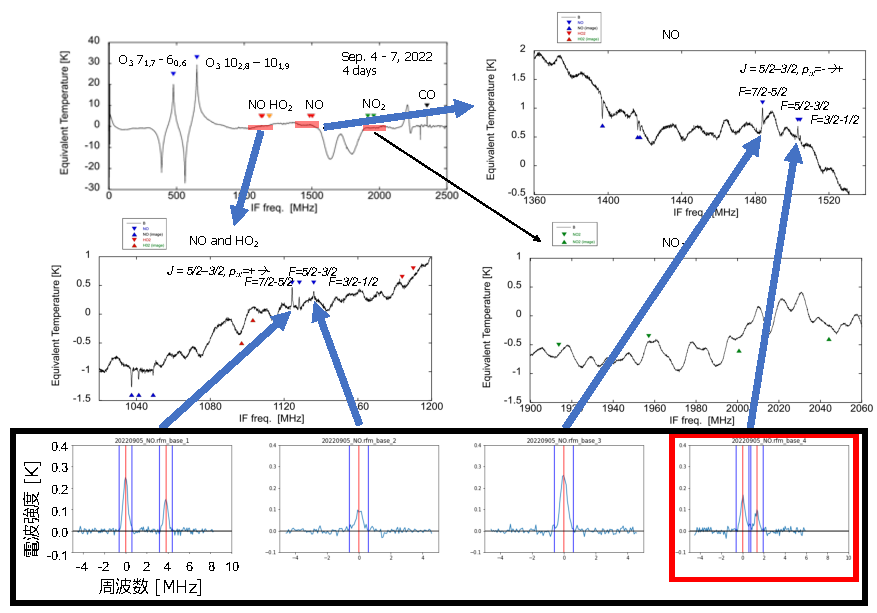
\includegraphics[width=\linewidth]{master_thesis_contents/master_thesis_fig/NO_spectr.pdf}
    % \caption{$\scriptstyle \mbox{昭和基地で現在観測できる6本の\ce{NO}輝線スペクトル} \scriptstyle
    % \mbox{(黒枠。赤枠はトロムソで観測できる2本の輝線スペクトル)}$}
    \caption{昭和基地で現在観測されている6本の\ce{NO}輝線スペクトルの例}
    % \caption{\protect 昭和基地で現在観測できる6本の\ce{NO}輝線スペクトル \linebreak
    % (黒枠。赤枠はトロムソで観測できる2本の輝線スペクトル)}
    \label{fig:NO_spectr}
\end{figure}
\begin{table}[htbp]
    \centering
    \caption{トロムソと昭和基地で観測される6本の\ce{NO}の輝線スペクトル}
    \label{tb:no_spectr_freq}
    \resizebox{\textwidth}{!}{%
    \begin{tabular}{cccccccc}
    \hline
    周波数 & \multicolumn{2}{c}{観測可能} & $J$ & $P_{\mathrm{ul}}$ & $F$ & IF 周波数  & 線スペクトル強度係数 $A$ \\
    $[\mathrm{GHz}]$ & Troms\o & Syowa &  &  &  & $[\mathrm{MHz}]$ & $[\mathrm{K^{-2}} \mathrm{MHz^{-1}} \mathrm{cm^{-2}}]$ \\ \hline
    $250.436848$ &  & $\circ$ & $5/2 - 3/2$ & \ce{+ -> -} & $7/2 - 5/2$ & $1124.3$ & $4.00\times 10^{13}$ \\ \hline
    $250.440659$ &  & $\circ$ & $5/2 - 3/2$ & \ce{+ -> -} & $5/2 - 3/2$ & $1128.2$ & $6.35\times 10^{13}$ \\ \hline
    $250.448530$ &  & $\circ$ & $5/2 - 3/2$ & \ce{+ -> -} & $3/2 - 1/2$ & $1136.0$ & $1.07\times 10^{14}$ \\ \hline
    $250.796436$ &  & $\circ$ & $5/2 - 3/2$ & \ce{- -> +} & $7/2 - 5/2$ & $1483.9$ & $3.99\times 10^{13}$ \\ \hline
    $250.815954$ & $\circ$ & $\circ$ & $5/2 - 3/2$ & \ce{- -> +} & $5/2 - 3/2$ & $1503.1$ & $6.33\times 10^{13}$ \\ \hline
    $250.816954$ & $\circ$ & $\circ$ & $5/2 - 3/2$ & \ce{- -> +} & $3/2 - 1/2$ & $1504.5$ & $1.06\times 10^{14}$ \\ \hline
    \end{tabular}%
    }
\end{table}
図\ref{fig:NO_spectr}を見ると、\ce{O3}スペクトルと比較して、\ce{NO}スペクトルはとても微弱である。
そのため、取得された全スペクトルデータのうち、どのデータが解析に用いることができるかということをあらかじめスクリーニングして抽出することが重要となる。


% \chapter{ミリ波観測解析手法}
\chapter{ミリ波観測のデータ解析}
\label{ch:mm_analysis}
\ref{ch:mm_obs}章で述べたように、トロムソは我々にとっては観測自体が初めての場所であり、昭和基地においては分光計を更新してから初めての観測である。
そのため、それぞれ観測装置の立ち上げ後に行われたテスト観測のデータを1つずつ精査した。
本章では、その手法と結果について述べる。\par

\ref{ssec:obs_syowa}節の図\ref{fig:NO_spectr}で示したように、\ce{NO}の輝線スペクトルはとても微弱である。
そのため、物理量の算出に十分なS/N比となるようにデータを処理し、輝線スペクトルを得る必要がある。
そこで今回は、全体のデータから設定した特定の条件をクリアした解析に用いることができるデータのみを選別する「スクリーニング」と、下層大気や観測装置の特性に起因する受信電波強度の補正を行った。
ミリ波分光計の観測システムは市販されているものではないため、ほぼ全てのハードウェア・ソフトウェアは自作となっており、今回用いるスクリーニングおよび電波強度の補正に必要なプログラムは自ら作成した。\par

スクリーニングと電波強度の補正については、以下のようにそれぞれ2つの観点から行った。
\begin{itemize}
    \item データのスクリーニング
    \begin{itemize}
        \item 光学的厚みの測定データを基にしたスクリーニング(\ref{sec:screening_opticaldepth}節)
        \item NOスペクトルデータのバックグラウンドノイズを基にしたスクリーニング(\ref{sec:screening_spectralnoise}節)
    \end{itemize}
    \item 電波強度の補正
    \begin{itemize}
        \item 下層大気の光学的厚みの影響の補正(\ref{sec:correction_opticaldepth}節)
        \item NOスペクトルデータのベースラインの補正(\ref{sec:correction_baselinefitting}節)
    \end{itemize}
\end{itemize} \par
本研究における解析を行うにあたって、トロムソでは2018年12月26日〜2019年3月10日の期間に行われたテスト観測のデータを用い、昭和基地では2023年3月22日〜2023年3月30日の観測データを用いた。
これらのスクリーニングを行った結果、本研究で用いたデータの解析期間はトロムソでは2019年1月23日〜2019年2月4日と2019年2月17日〜2019年2月20日、南極・昭和基地では2023年3月22日〜2023年3月30日となった。
両極域での比較という観点では、トロムソ・昭和基地両方において同時期の観測データを用いるのが望ましい。
しかしながら、トロムソにおいて\today 時点で使用可能なデータは今回用いる期間のもののみであり、この時期における昭和基地は観測条件が悪く、解析に用いることができるデータを得ることができなかった。
そのため、今回は異なる時期での解析を行ったことに注意してほしい。
以下では、それぞれの解析手法とその結果について順番に述べて、\ref{sec:derive_columndensity}節は\ce{NO}の柱密度の導出について述べる。


\section{光学的厚みの測定データを基にしたスクリーニング}
\label{sec:screening_opticaldepth}
\ref{ssec:obs_opticaldepth}節で述べたように、ミリ波分光計を用いた中層大気(主に上部成層圏〜下部熱圏)の地上観測では、下層大気(主に対流圏)による影響を受けるため、観測中定期的に実測する光学的厚みの測定データを用いて、この影響を取り除いている。
光学的厚みの測定を行っている間に大気分子の観測を行っているため、光学的厚みは大気分子の観測を行っている間、安定しているという前提の上で光学的厚みによる電波強度の補正を行っている。
従って、光学的厚みの測定データは観測データに対して充分に安定していなければならない。\par

図\ref{fig:optical_depth_tromsoe}に示しているデータは、トロムソの観測装置立ち上げ後に行われたテスト観測の期間に測定された光学的厚みの時間変化を表したものである。
\begin{figure}[htbp]
    \centering
    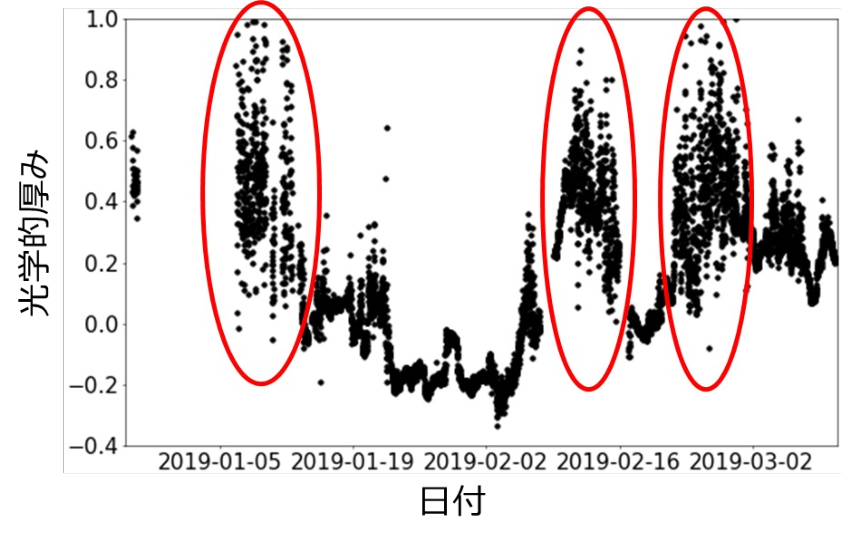
\includegraphics[width=\linewidth]{master_thesis_contents/master_thesis_fig/optical_depth_tromsoe.pdf}
    \caption{トロムソでの光学的厚み測定データの時間変化(~\cite{goto2021bachelor}より引用)}
    \label{fig:optical_depth_tromsoe}
\end{figure}
比較的値が安定している時期と、値が大きくばらついて安定していない時期がある(例として赤丸で示す)。
この赤丸で示された時期は、光学的厚みの典型値(たとえば南極昭和基地ではおよそ$0.1-0.4$の範囲の値をとる)とは大きく外れている。
% 何に基づく典型値でしょうか?先行研究で示されているものであれば、それを引用。
このように短時間で値の変動が大きい場合は、光学的厚みが測定される時間スケール(測定間隔はおよそ$12-13$分)で、下層大気の影響が変化しており一様でないことを表している。
そのため、離散的に測定された光学的厚みの値を用いて、その間に観測されたスペクトルデータの電波強度を一様に補正するには適さないと考えられる。\par

そこでまず、観測データの強度の補正に使用できる光学的厚みのデータを決定するために、光学的厚みの測定したデータそれ自体のスクリーニングを行うことを考えた。
このスクリーニングで残った期間の観測データを後の解析に用いることとする。\par

スクリーニング方法としては、まず1日ごとにデータを区切り
% (一日の間で測定される光学的厚みのデータ数は**個程度になる)
、それぞれの日でこれらの分散を計算し、その分散が$0.005$以下の値の日をとるデータを使用することとした。
分散の閾値を0.005としたのは、図\ref{fig:optical_depth_tromsoe}のデータを目視し、値が安定していると判断した2019年1月23日〜2019年2月4日の分散がいずれも0.005以下であったため、このように設定した~\cite{goto2021bachelor}。
この条件を設定することで、光学的厚みの変動が大きい、すなわち下層大気の影響が過度に大きく、データの質が安定しない時間帯を除去することができる。
南極・昭和基地の解析においても同条件でスクリーニングを行った。
% この章は、既に本研究の結果を示す章なので、南極のデータも具体的に示す。


\section{NOスペクトルデータのバックグラウンドノイズを基にしたスクリーニング}
\label{sec:screening_spectralnoise}
次に、\ref{sec:screening_opticaldepth}節のスクリーニングで残った\ce{NO}スペクトルの観測データにおいて、解析に使うことのできない質の悪いデータをスクリーニングすることを考える。
トロムソの観測期間の全取得データを精査した結果、スペクトルデータに含まれる顕著なノイズ成分というのは、周波数的に非常に狭く強度の強いスパイク状のノイズと、全体に渡ってランダムな強いノイズの2種類があることがわかった~\cite{goto2021bachelor}。
そこで、これらのスパイク状のノイズと全体的なノイズをそれぞれ自動的に判別する条件を決めることで、図\ref{fig:raw_spectrum}(a)のような質の良いデータのみを抽出することを目指す。\par

まず、NOスペクトルが存在する周波数($250.435-250.817\ \mathrm{GHz}$)を含む分光計の$5000-10000$チャンネルの範囲のデータに対し、二次曲線をフィッティングした。
この周波数帯にランダムノイズがどれだけ含まれているか調べるために、この近似値に対する測定値の二乗平均誤差を計算する。
ここでは$5000-10000$チャンネルにおいてスペクトルデータの典型的なベースラインの形状が二次関数的であったため、二次近似を用いることにした(図\ref{fig:raw_spectrum}(a)の赤線)。
\begin{figure}[htbp]
    \centering
    \begin{minipage}{0.33\linewidth}
        \centering
        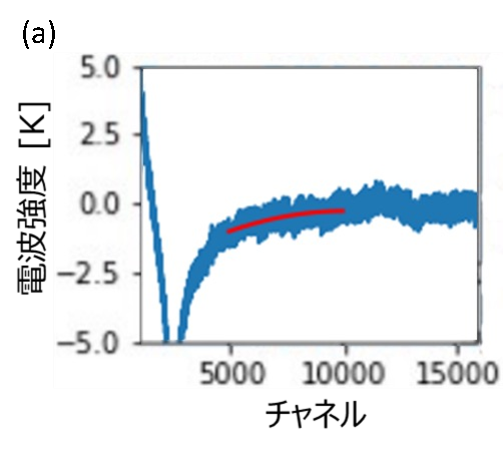
\includegraphics[width=\linewidth]{master_thesis_contents/master_thesis_fig/raw_spectrum_good.pdf}
    \end{minipage}
    \begin{minipage}{0.6\linewidth}
        \centering
        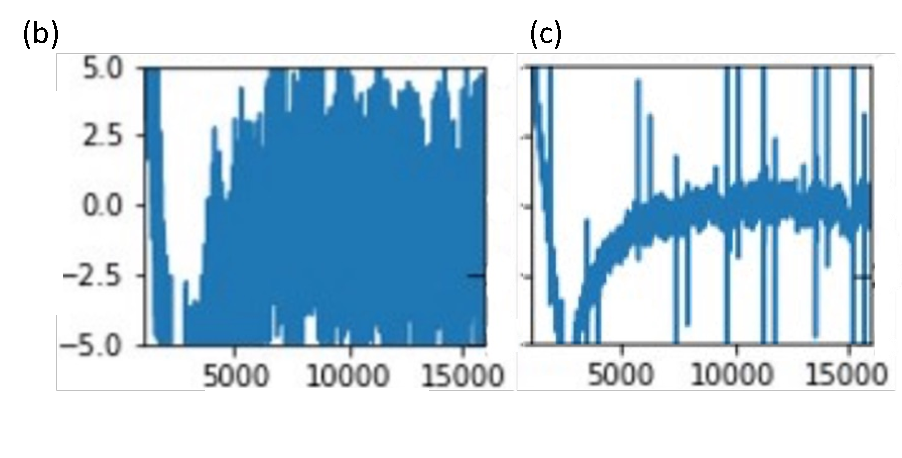
\includegraphics[scale=0.6]{master_thesis_contents/master_thesis_fig/raw_spectrum_bad.pdf}
    \end{minipage}
    \caption{(a) 解析に用いるために望ましい生データの一例($5000\, \mathrm{ch}$以下のデータは$239.093279\, \mathrm{GHz}$のオゾンの放射スペクトルデータがFRSWにより反映された結果、赤線は$5000-10000\, \mathrm{ch}$でのスペクトルデータの近似二次曲線を表す。)。(b)(c) スクリーニングしたいデータの例((b)は全体的にノイズを含む例、(c)はスパイク状のノイズを含む例を表す)。}
    \label{fig:raw_spectrum}
\end{figure}
この結果から、スクリーニング条件としては以下の2つを設定した~\cite{goto2021bachelor}。
\begin{itemize}
    \item 2乗平均誤差の整数丸め値が0ではない
    \item $5000-10000$チャンネルで強度の絶対値が$5\, \mathrm{K}$以上の値を含む
\end{itemize} \par
1つ目の条件は、全体的にノイズを含むデータ(たとえば図\ref{fig:raw_spectrum}(b))を判別・除去することを意図しており、2つ目の条件はスパイク状のノイズを含むデータ(たとえば図\ref{fig:raw_spectrum}(c))を除去することを意図している。
設定したスクリーニング条件が妥当かどうかの検証は、既に卒業研究~\cite{goto2021bachelor}にて行っている。
卒業結果では、明らかにノイズを含むデータについては意図した通りにスクリーニングをすることができており、質のよいデータのみを選ぶことに成功したという結論を得ている。
% このあとに節を追加し、南極昭和基地についても結果を述べる。


\section{トロムソにおける光学的厚みの測定データの異常値の検討}
\label{sec:correction_opticaldepth}
\ref{sec:screening_opticaldepth}節に述べたように、光学的厚みが短時間で変動している不安定なデータを除去したことによって、トロムソの観測データについては図\ref{fig:optical_depth_minus}のように期間A(2019年1月23日〜2019年2月4日)と期間B(2019年2月17日〜2019年2月20日)が残った。
しかし、期間Aにおいて光学的厚みが$-0.2$程度と負の値となっていることがわかった(図\ref{fig:optical_depth_minus}の赤丸)。
\begin{figure}[htbp]
    \centering
    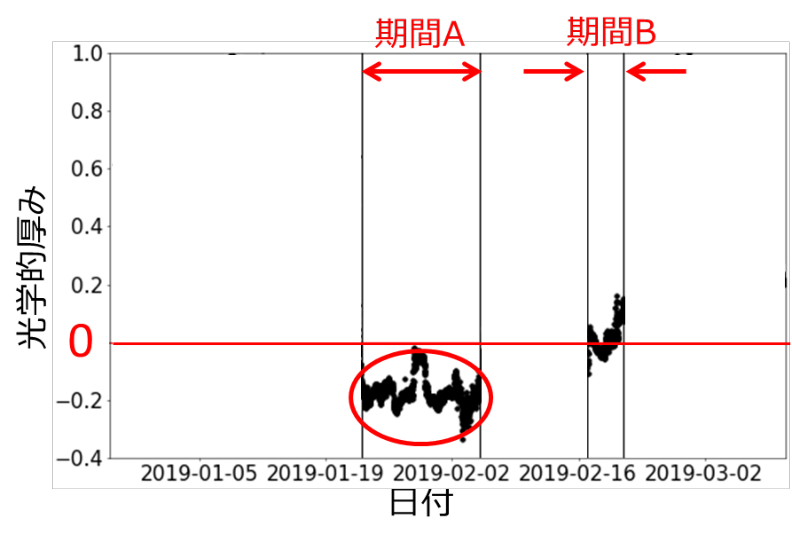
\includegraphics[width=\linewidth]{master_thesis_contents/master_thesis_fig/optical_depth_minus.pdf}
    \caption{トロムソにおいて負の値をとる光学的厚み(~\cite{goto2021bachelor}より引用)}
    \label{fig:optical_depth_minus}
\end{figure}
\ref{ch:mm_obs}章で述べた光学的厚みの算出方法のことを考えると、この値が負の値を取ることはない。
そこでこの原因を調べたところ、光学的厚みを算出する際に使用する式\eqref{eq:opticaldepth_plot}におけるプロットデータにおいて、各観測天頂角$z$における$\sec z$に対する$\ln \left( T_{obs\_ hot} - T_z \right)$が、もっとも観測天頂角が小さい($\sec z$が1番小さい)ところで異常に低くなっていた。
これによってフィッティングされた近似直線の傾きが正になってしまうことで、光学的厚みが負の値として計算されていることが分かった~\cite{goto2021bachelor}。
その模式図を図\ref{fig:optical_depth_slope_minus}、実際の測定データ例を図\ref{fig:optical_depth_measurement_good_bad}に示す。\par

\begin{figure}[htbp]
    \centering
    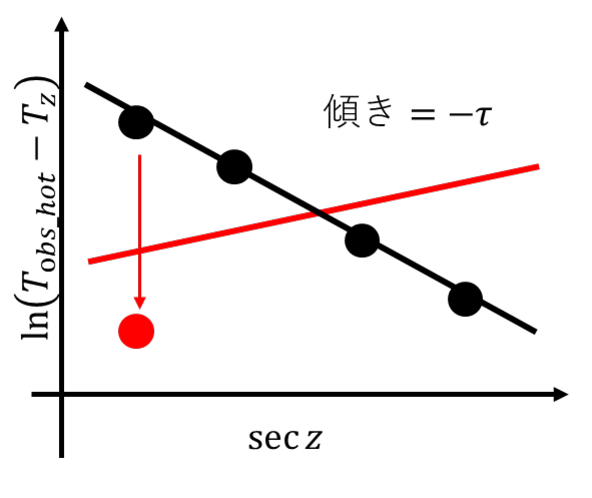
\includegraphics{master_thesis_contents/master_thesis_fig/optical_depth_slope_minus.pdf}
    \caption{プロットデータの落ち込みによる光学的厚みの計算値の変化(プロットデータの落ち込みにより近似直線が黒線→赤線に変わり、直線の傾きが変わる)~\cite{goto2021bachelor}より引用。}
    \label{fig:optical_depth_slope_minus}
\end{figure}
\begin{figure}[htbp]
    \centering
    \begin{minipage}{0.41\linewidth}
        \leftline{(a)}
        \centering
        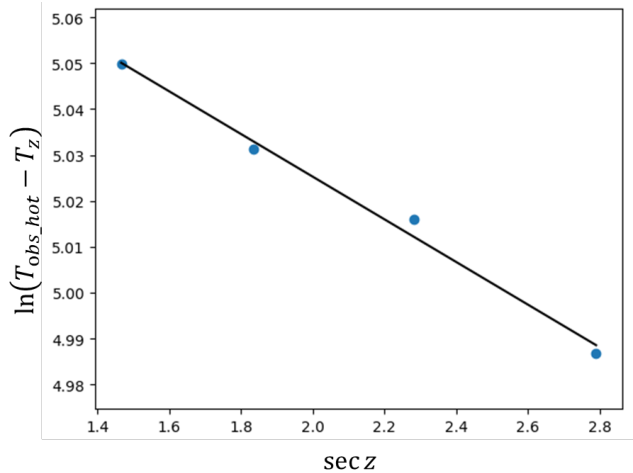
\includegraphics[width=\linewidth]{master_thesis_contents/master_thesis_fig/optical_depth_good.pdf}
    \end{minipage}
    \begin{minipage}{0.45\linewidth}
        \leftline{(b)}
        \centering
        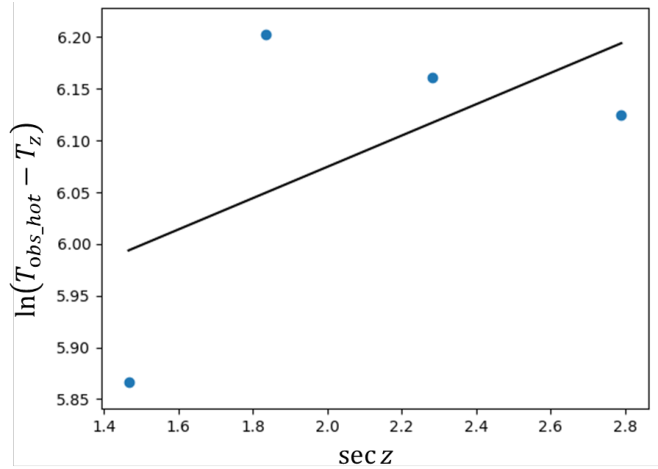
\includegraphics[scale=0.6]{master_thesis_contents/master_thesis_fig/optical_depth_bad.pdf}
    \end{minipage}
    \caption{(a) 望ましいプロットデータの一例(2019年2月17日5時51分頃測定)。(b) プロットデータが落ち込んだ実際のデータの一例。(2019年1月23日0時5分頃測定)。黒線は近似直線を表す。~\cite{goto2021bachelor}より引用。}
    \label{fig:optical_depth_measurement_good_bad}
\end{figure}
さらに、その天頂角が最も小さいデータの落ち込みの原因を調べたところ、この光学的厚みの値が負の値となっている期間の終わりごろに、光学的厚みの測定で用いる観測方向(\ref{ssec:obs_opticaldepth}節の表\ref{tb:secz_zdeg})にあるコンテナー側面の観測窓の上部に氷柱ができているのを見つけたという報告があり(図\ref{fig:icicles})、それが時期的に一致していることが分かった~\cite{goto2021bachelor}。
\begin{figure}[htbp]
    \centering
    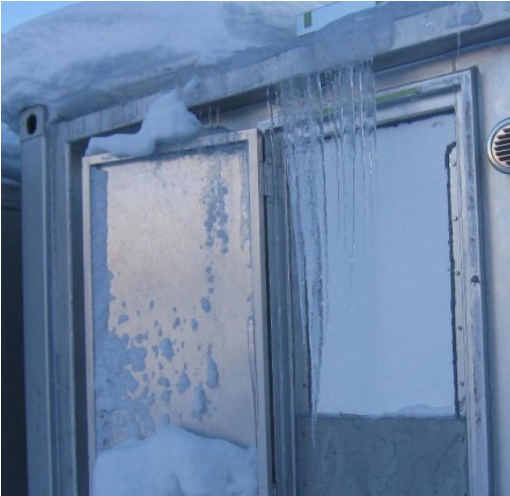
\includegraphics[width=\linewidth]{master_thesis_contents/master_thesis_fig/icicles.pdf}
    \caption{側窓にできた氷柱(~\cite{goto2021bachelor}より引用)}
    \label{fig:icicles}
\end{figure}
したがって、天頂角がもっとも小さい角度で測定された電波強度は、この氷柱の影響を受けてしまった可能性があると考えられる。
従ってこの期間は、天頂角のもっとも小さい方向の測定データは用いずに光学的厚みを算出することにした。
この妥当性の検証は卒業研究~\cite{goto2021bachelor}にて既に行っている。
卒業研究では、氷柱の影響を受けたとみられる期間において、光学的厚みの補正ができており、氷柱が除去された期間においては本来の値とほぼ一致しているため補正せずに用いることができるという結論を得ている。


\section{NOスペクトルデータのベースラインの補正}
\label{sec:correction_baselinefitting}
\ref{sec:screening_opticaldepth}節や\ref{sec:screening_spectralnoise}節によるスクリーニングで残った期間における\ce{NO}スペクトルデータについて、積分を行う。
昭和基地で行われた先行研究であるIsonoらによるデータ解析の結果~\cite{isono2014ground}より、24時間の積分をすることで十分なS/N比が得られることが示されている。
積分したスペクトルデータには、観測対象である\ce{NO}の輝線スペクトルだけでなく、下層大気や装置由来の連続波成分が含まれているため、ベースラインの補正を行う必要がある。
本研究では、\ce{NO}スペクトルから外れた両端におけるデータがバックグラウンドの成分を表していると考え、これをベースラインとして近似から求め、元のスペクトルから差し引くことにした。
これにより、FRSWで除去しきれなかったオフセット成分や周波数特性のうねりなどが除去され、観測対象の\ce{NO}スペクトルのみを取り出すことができる。\par

ベースラインの補正の模式図を図\ref{fig:baseline_correct_schema}に示す。
\begin{figure}[htbp]
    \centering
    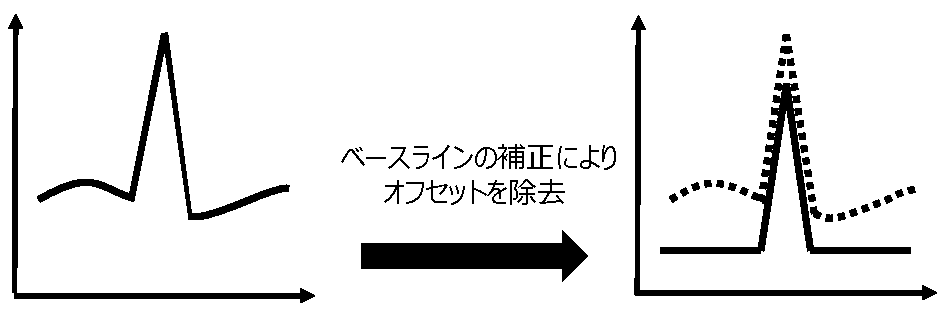
\includegraphics[width=\linewidth]{master_thesis_contents/master_thesis_fig/baseline_correct_schema.pdf}
    \caption{ベースライン近似を用いたベースラインの補正}
    \label{fig:baseline_correct_schema}
\end{figure}
ベースラインの近似に用いるデータは、図\ref{fig:baseline_range}の赤色で示した\ce{NO}スペクトルの両端のそれぞれ$5\, \mathrm{MHz}$の範囲を使用した。
この範囲は、対象とするNOの放射スペクトル成分が含まれないと考えられる。
\begin{figure}[htbp]
    \centering
    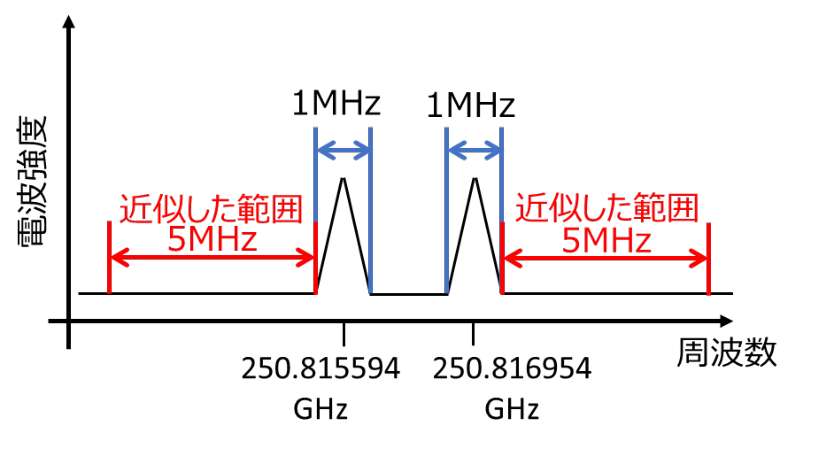
\includegraphics[width=\linewidth]{master_thesis_contents/master_thesis_fig/baseline_range.pdf}
    \caption{ベースラインを補正する元となる周波数の範囲(赤色で表示。青色は検出するスペクトルの幅を示している。例としてトロムソで用いた2本の輝線スペクトルの場合を示した。)}
    \label{fig:baseline_range}
\end{figure}
スペクトルデータを見ると、この周波数帯では典型的なベースラインの形状が、図\ref{fig:baseline_curve}に示す赤い曲線のような三次関数的な形であったので、ここでは三次関数で近似を行うことにした。
\begin{figure}[htbp]
    \centering
    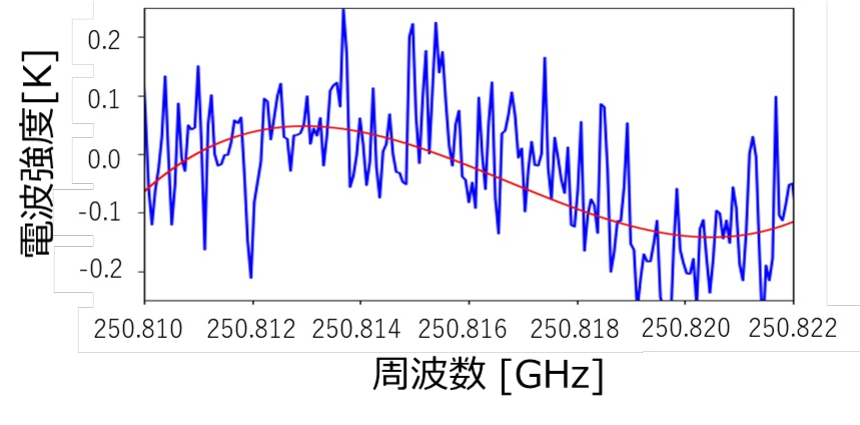
\includegraphics[width=\linewidth]{master_thesis_contents/master_thesis_fig/baseline_curve.pdf}
    \caption{三次関数的な形のベースライン(~\cite{goto2021bachelor}より引用)}
    \label{fig:baseline_curve}
\end{figure}
また、\ce{NO}の各スペクトル幅は$1\, \mathrm{MHz}$と仮定した。
このように仮定したのは対象の時期の日ごとのデータにおいて、放射スペクトルの幅の大きさがどの日のデータにおいてもおよそ$1\, \mathrm{MHz}$であることが確認できたためである(図\ref{fig:no_spectr_exp}にあるデータの一例においても、\ce{NO}スペクトル根本での幅がおよそ$1\, \mathrm{MHz}$であることが確認できる)。
% このあと、南極のデータについても説明
\begin{figure}[htbp]
    \centering
    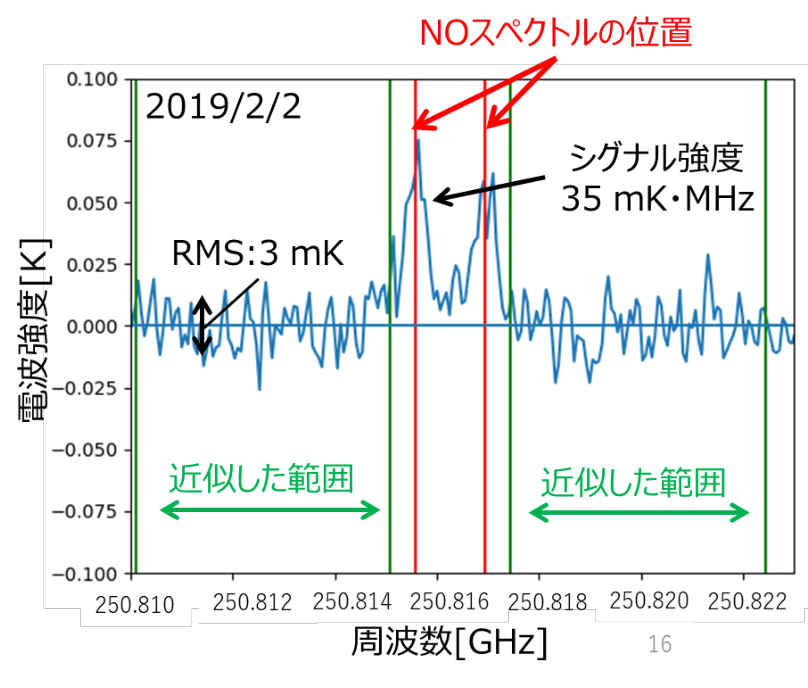
\includegraphics[width=\linewidth]{master_thesis_contents/master_thesis_fig/no_spectr_exp.pdf}
    \caption{スペクトルの検出の一例。2019年2月2日おける24時間積分によるスペクトルデータの一例。赤線は検出するスペクトルがある周波数の位置、緑線はベースライン近似に用いたスペクトルデータの範囲を示す。赤線と一番近くにある緑線の間が輝線スペクトルピークから端の間($=0.5\ \mathrm{MHz}$)にあたる。シグナル強度とRMSについては柱密度の導出(\ref{sec:derive_columndensity}節)で用いる(~\cite{goto2021bachelor}より引用)}
    \label{fig:no_spectr_exp}
\end{figure}
\clearpage


\section{NO柱密度(Column Density)の導出}
\label{sec:derive_columndensity}
柱密度とは高度方向に密度を足し合わせたものであり、
今回はスペクトルの線形から$70\, \mathrm{km}$以上に存在する\ce{NO}分子についてみたものとなる。
% これの理由が不明確ですので、説明をすること。
まず、本研究で用いたそれぞれの輝線スペクトルにおいて柱密度の導出を行った。
柱密度の導出方法は、先行研究~\cite{isono2014ground}を参考にして行った。
導出に用いた式は以下である。
\begin{gather}
    N_{\mathrm{NO}} = A \times T_{\mathrm{atm}} \times \int T_{\mathrm{NO}}d\nu
    \label{eq:derive_columndensity} \\
    N_{\mathrm{NO}}:\ce{NO}の柱密度[\mathrm{cm^{-2}}]、A:線スペクトル強度係数[\mathrm{K^{-2}} \cdot \mathrm{MHz^{-1}} \cdot \mathrm{cm^{-2}}] \notag \\
    T_{\mathrm{atm}}:大気温度[\mathrm{K}]、\int T_{\mathrm{NO}}d\nu:\ce{NO}のスペクトル積分強度 \notag
\end{gather} \par
線スペクトル強度係数は、分子・周波数ごとに決まる値となる。
柱密度は、理想的にはどの輝線スペクトルからも、等しい柱密度の値に求まる必要がなる。
線スペクトル強度係数は、その値を調整するための役割としてのパラメーターとなる。
本研究で用いた\ce{NO}の輝線スペクトルにおけるそれぞれの線スペクトル強度係数は、\ref{ssec:obs_syowa}節の表\ref{tb:no_spectr_freq}に記載している。
\ref{ssec:obs_syowa}節でも述べたが、線スペクトル強度係数は、NASAが提供しているJPL Catalogより調べた。
大気温度は一様に$200\, \mathrm{K}$と仮定し、\ce{NO}は光学的に薄いと仮定している。
また、トロムソに設置された観測装置はDSBミクサを用いているため(\ref{sec:obs_location}節の表\ref{tb:spectrometer_spec})、\ref{ssec:obs_overview}節で述べたように輝線スペクトル強度については実際の観測データから計算したものに2倍した値を用いている。
柱密度の誤差は、\ref{sec:correction_baselinefitting}節で述べたベースライン近似の際に用いたチャンネル範囲におけるRMS(Root Mean Square)を用いて、式\refeq{eq:derive_columndensity}と同様の方法で求めた。
式を以下に示す。
\begin{gather}
    \varepsilon = \pm A \times T_{\mathrm{atm}} \times \int T_{\mathrm{rms}}d\nu \\
    T_{\mathrm{rms}}:\mathrm{RMS[K]} \notag
\end{gather} \par
次にそれぞれの輝線スペクトルにおいて導出した柱密度についての平均を計算した。
柱密度の平均値については、それぞれの輝線スペクトルの柱密度を導出する際に用いた線スペクトル強度係数によって重み付けをした。
線スペクトル強度係数による重み付けの平均の式を以下に示す。
\begin{gather}
    N_{\mathrm{avg}} = \left. \sum_{k} \frac{N_{k}}{\left| \varepsilon_{k}\right|} \middle/ \sum_{k} \frac{1}{\left| \varepsilon_{k}\right|} \right. \\
    N_{\mathrm{avg}}:\ce{NO}の平均柱密度、N_{\mathrm{k}}:一つの輝線スペクトルから導出した柱密度 \notag \\
    \varepsilon_{\mathrm{k}}:一つの輝線スペクトルから導出した柱密度の誤差 \notag
\end{gather} \par
また、柱密度の誤差についても以下のように同様に重み付けによる平均を計算した。
\begin{equation}
    \varepsilon_{\mathrm{avg}} = \pm \left( \sum_{k} \frac{1}{\left| \varepsilon_{k}\right|} \right)^{-1}
\end{equation}


% \chapter{結果}
\chapter{結果}
\label{ch:results}
\ref{ch:results}章では、\ref{ch:mm_analysis}章で紹介した手法を踏まえて導出した柱密度の結果について述べていく。
まず、トロムソと昭和基地で共通してわかったこととしては、どちらとも\ce{NO}の短期的変動が確認できたことである。
以降、トロムソ(\ref{sec:results_tromsoe}節)と昭和基地(\ref{sec:results_syowa}節)と観測場所別に分けて述べていく。

\section{ノルウェー・トロムソでの解析結果}
\label{sec:results_tromsoe}
スクリーニングの結果、2つの期間が残った。
1つ目の期間は、2019年1月23日〜2019年2月4日、2つ目の期間は2019年2月17日〜2019年2月20日となった。
参考として2つの期間の間の時間変動を確認するため、本来スクリーニングされた期間(2019年2月5日〜2019年2月16日)についてもプロットした(図\ref{fig:avg_ColumnDensity_tromsoe}のグレーのエラーバー)。
時間分解能は24時間となり、プロット間隔も24時間(1日1プロット)とした。
\begin{figure}[htbp]
    \centering
    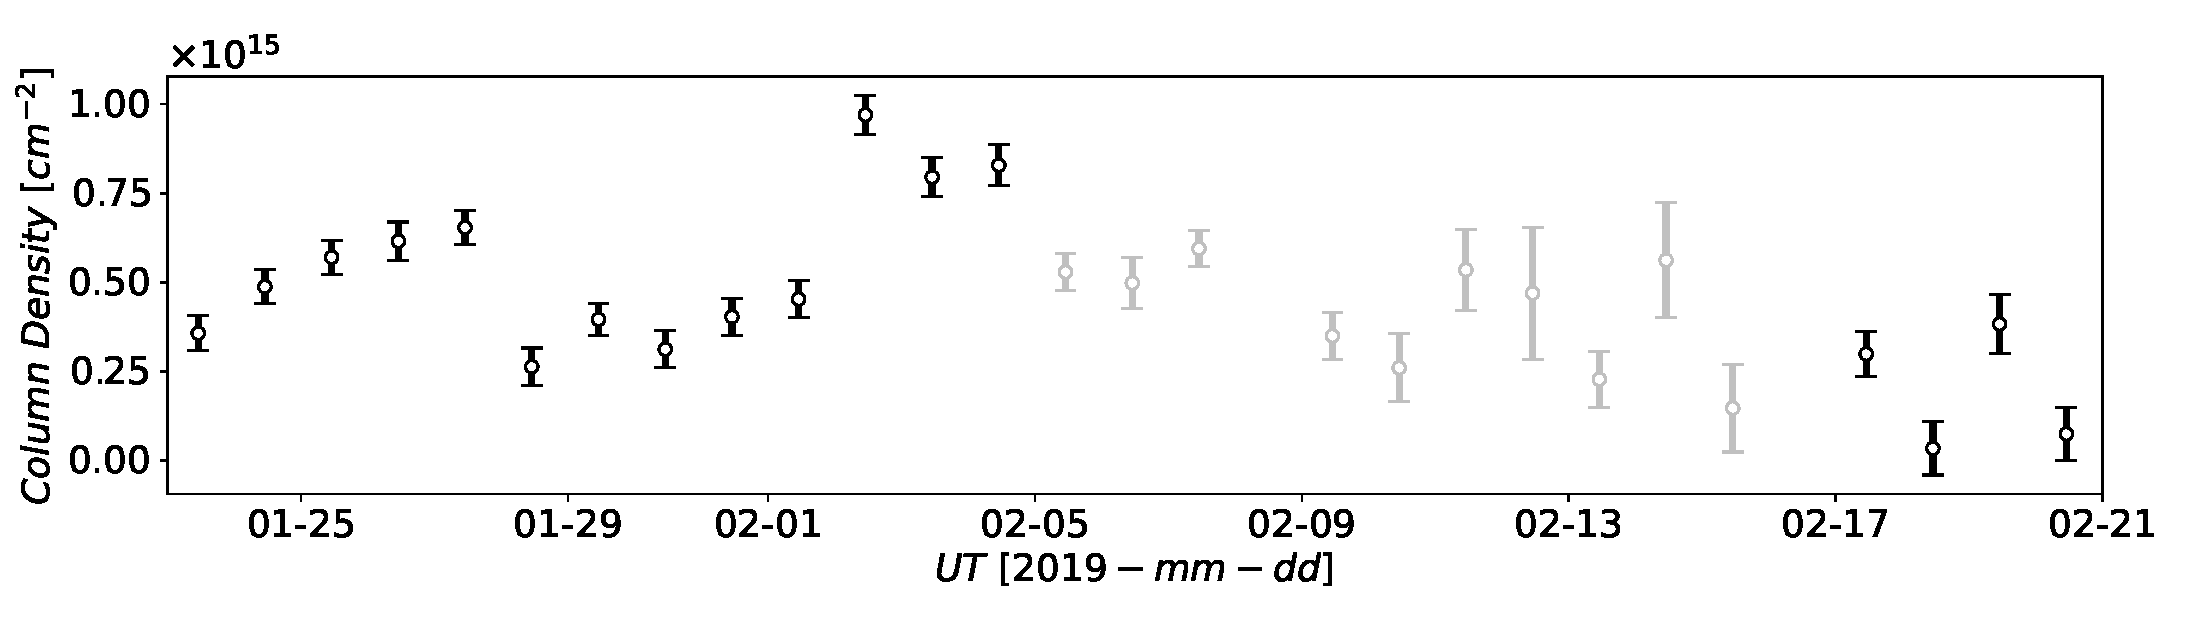
\includegraphics[width=\linewidth]{master_thesis_contents/master_thesis_fig/avg_ColumnDensity_tromsoe.pdf}
    \caption{トロムソにおける\ce{NO}柱密度の時間変動(グレーのエラーバーは本来スクリーニングされた期間であることを示す)}
    \label{fig:avg_ColumnDensity_tromsoe}
\end{figure}
\ce{NO}の柱密度について、エラーバーの範囲を超える有意な増加がみられる期間が2つあった(2019年1月23日〜2019年1月27日と2019年2月1日〜2019年2月4日)。
1つ目の時期(2019年1月23日〜2019年1月27日)16\% の緩やかな増加となり、2つ目の時期(2019年2月1日〜2019年2月4日)は83\% の急激な増加が確認できた。


\section{南極・昭和基地での解析結果}
\label{sec:results_syowa}
スクリーニングの結果、2023年3月22日〜2023年3月30日の期間が残った。
昭和基地ではNOの6本の超微細構造線を全て用いることで、積分時間は12時間とし、プロット間隔は6時間とした。
その結果、柱密度の誤差の平均は、積分時間が24時間であるトロムソの解析結果(\ref{sec:results_tromsoe}節の図\ref{fig:avg_ColumnDensity_tromsoe})と比べて20\% 小さくすることができ、時間分解能は12時間と良くなった。
\ce{NO}の柱密度について、エラーバーの範囲を超える有意な増加がみられる期間が2つあった(2023年3月23日21時〜2023年3月24日3時と2023年3月25日9時〜2023年3月25日21時)。
どちらも1プロットごとに増加となった。
\begin{figure}[htbp]
    \centering
    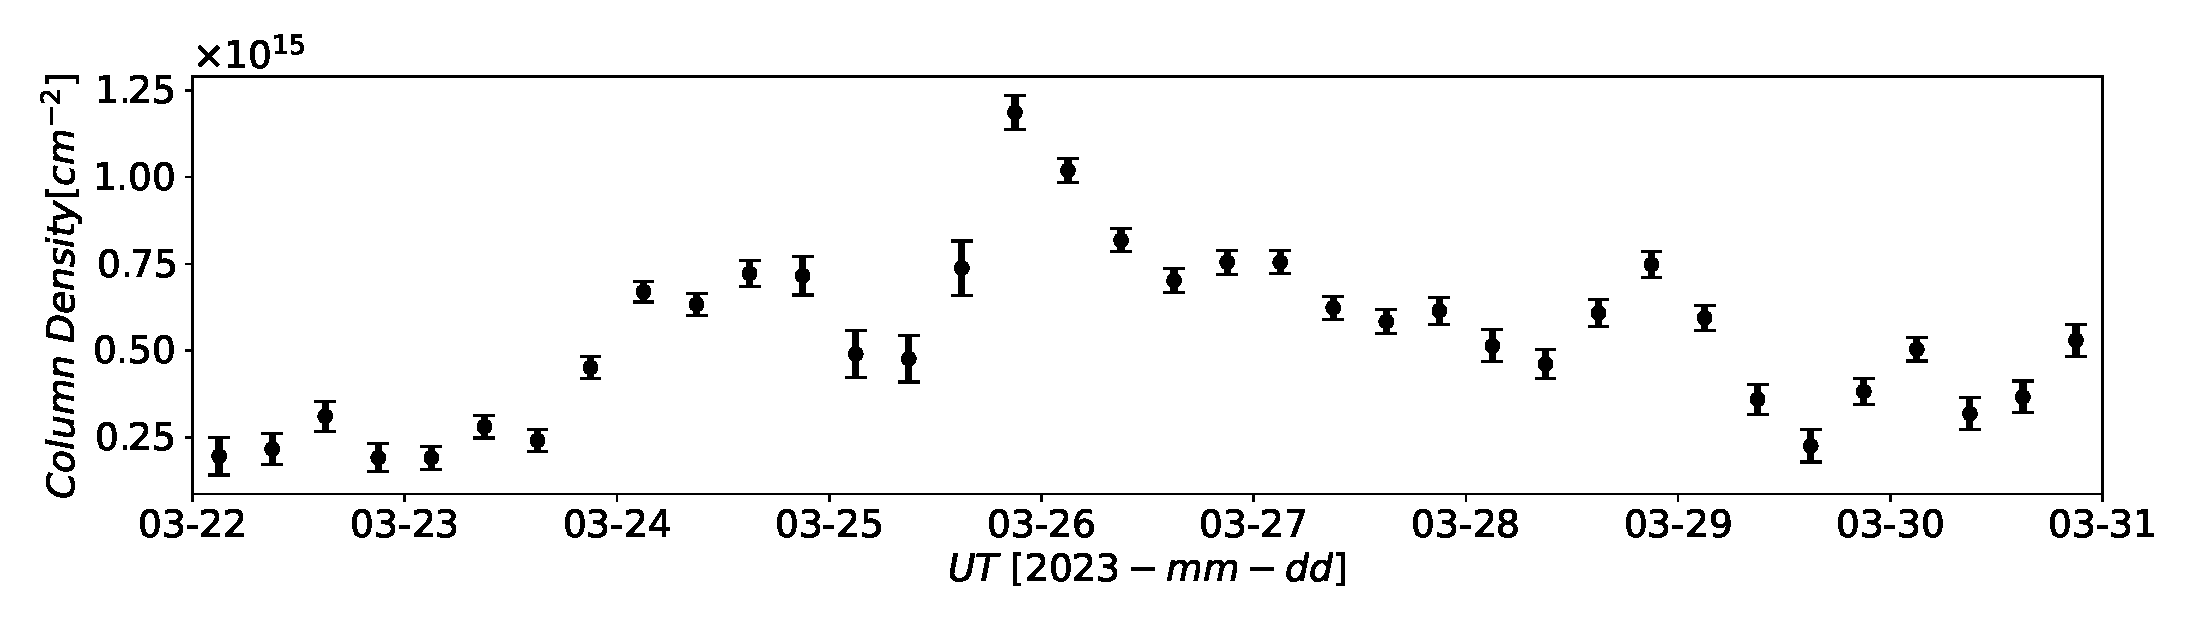
\includegraphics[width=\linewidth]{master_thesis_contents/master_thesis_fig/column_density_spectr6_syowa.pdf}
    \caption{昭和基地における\ce{NO}柱密度の時間変動}
    \label{fig:column_density_spectr6_syowa}
\end{figure}


% \chapter{考察}
\chapter{考察}
\label{ch:discussion}
\ref{ch:discussion}章では\ref{ch:results}章での結果との比較とを行う。
\ref{sec:comparison_sofie}節では、ノルウェー・トロムソにおける解析結果(\ref{sec:results_tromsoe}節)において、SOFIE: Solar Occultation for Ice Experiment(詳細は付録\ref{app:sofie})によって観測データを用いた比較を行う。
\ref{sec:comparison_eep}節では、POES/MetOp: Polar Orbiting Environmental Satellites/Meteorological Operational Satellite(詳細は付録\ref{app:poes})衛星の観測によるデータおよびNASAが提供しているOMNI Web Dataを用いて比較を行う。


\section{SOFIEデータによって導出されたNO柱密度との比較}
\label{sec:comparison_sofie}
まずは、ミリ波分光計を用いた\ce{NO}の観測データの妥当性を確認するため、SOFIEによる\ce{NO}の高度プロファイルデータを用いた。
今回、トロムソの柱密度を導出した期間と同じ時期にトロムソ付近の緯度(およそ65 - 80\textdegree Nの範囲)で観測されたSOFIEのデータを用いた。
その比較結果を図\ref{fig:sofie_mmcd}に示す。
\begin{figure}[htbp]
    \centering
    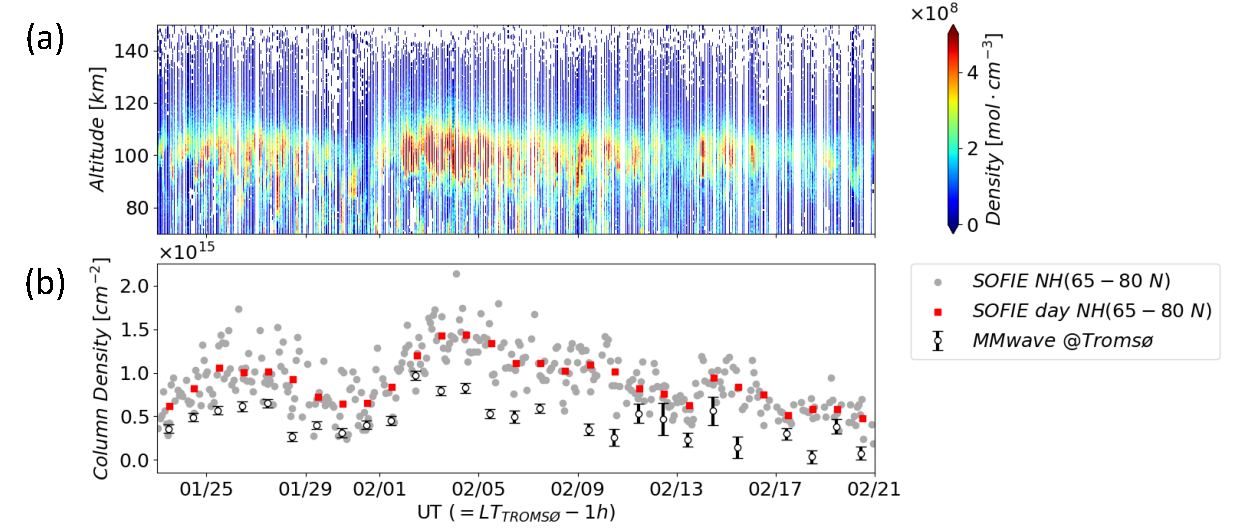
\includegraphics[width=\linewidth]{master_thesis_contents/master_thesis_fig/sofie_mmcd.pdf}
    \caption{(a)SOFIEのNO高度プロファイルデータおよび(b)ミリ波分光計を用いて導出したトロムソの柱密度とSOFIEの高度プロファイルデータから導出した柱密度の比較(エラーバー付きのプロットがミリ波データから導出した柱密度、グレーの丸形プロットがSOFIEの高度プロファイルデータから導出した柱密度、赤色の四角プロットが1日平均したSOFIEの柱密度)}
    \label{fig:sofie_mmcd}
\end{figure}



\section{高エネルギー電子の降り込みとの比較}
\label{sec:comparison_eep}
電子フラックス

% \begin{figure}[htbp]
%     \centering
%     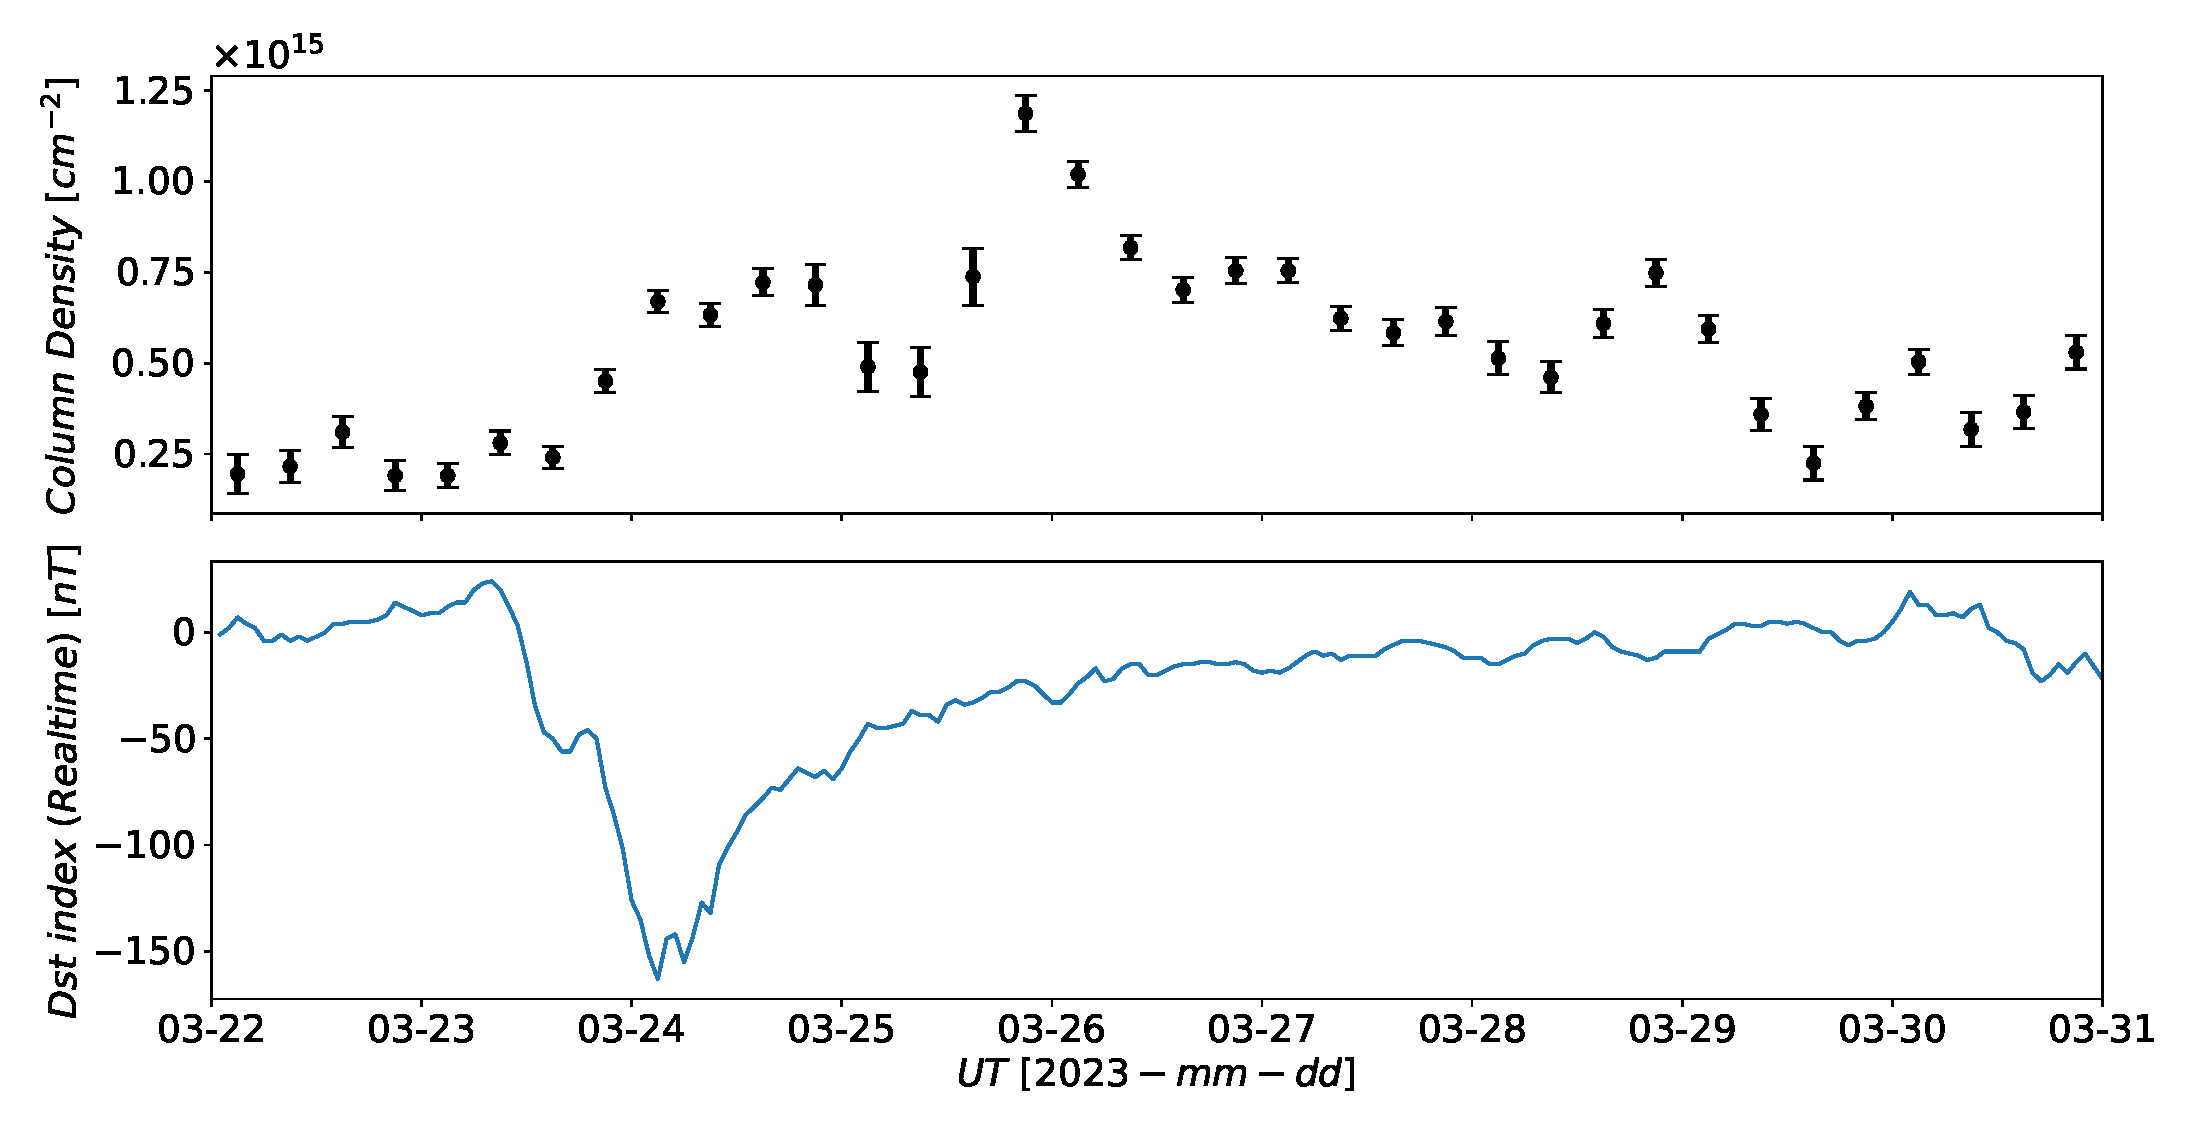
\includegraphics[width=\linewidth]{master_thesis_contents/master_thesis_fig/column_density_spectr6_dst_syowa.pdf}
%     \caption{昭和基地における柱密度(1段目。図\ref{fig:column_density_spectr6_syowa}と同じ)とDst指数(2段目)との比較}
%     \label{fig:dst_mmcd_syowa}
% \end{figure}
% Dst指数のグラフ
\begin{figure}[htbp]
    \centering
    \begin{minipage}{\linewidth}
        \centering
        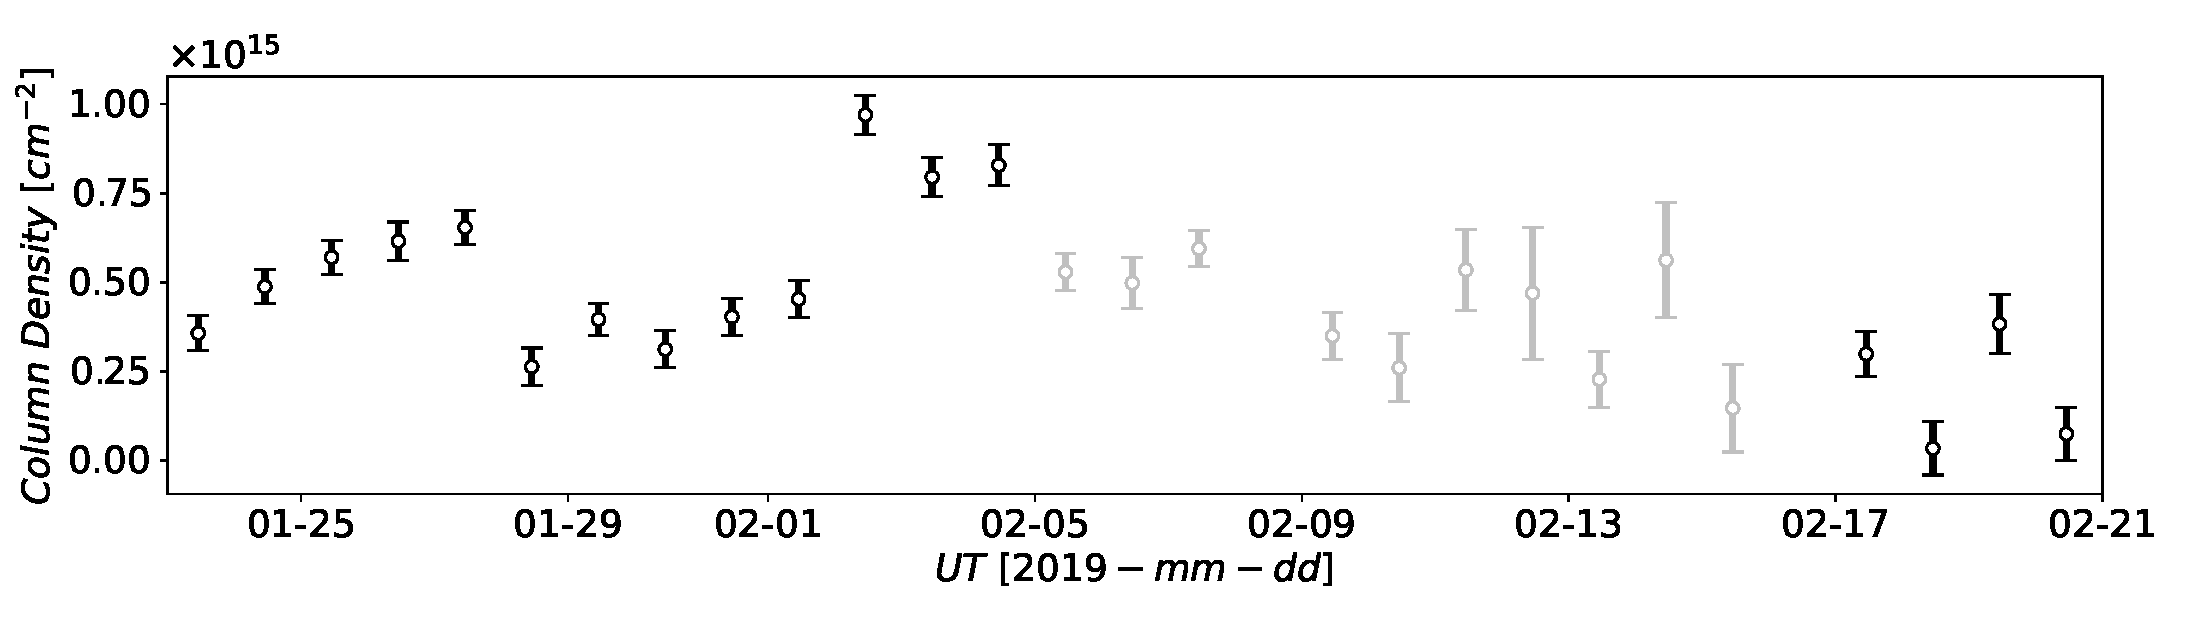
\includegraphics[width=\linewidth]{master_thesis_contents/master_thesis_fig/avg_ColumnDensity_tromsoe.pdf}
    \end{minipage}
    \begin{minipage}{\linewidth}
        \centering
        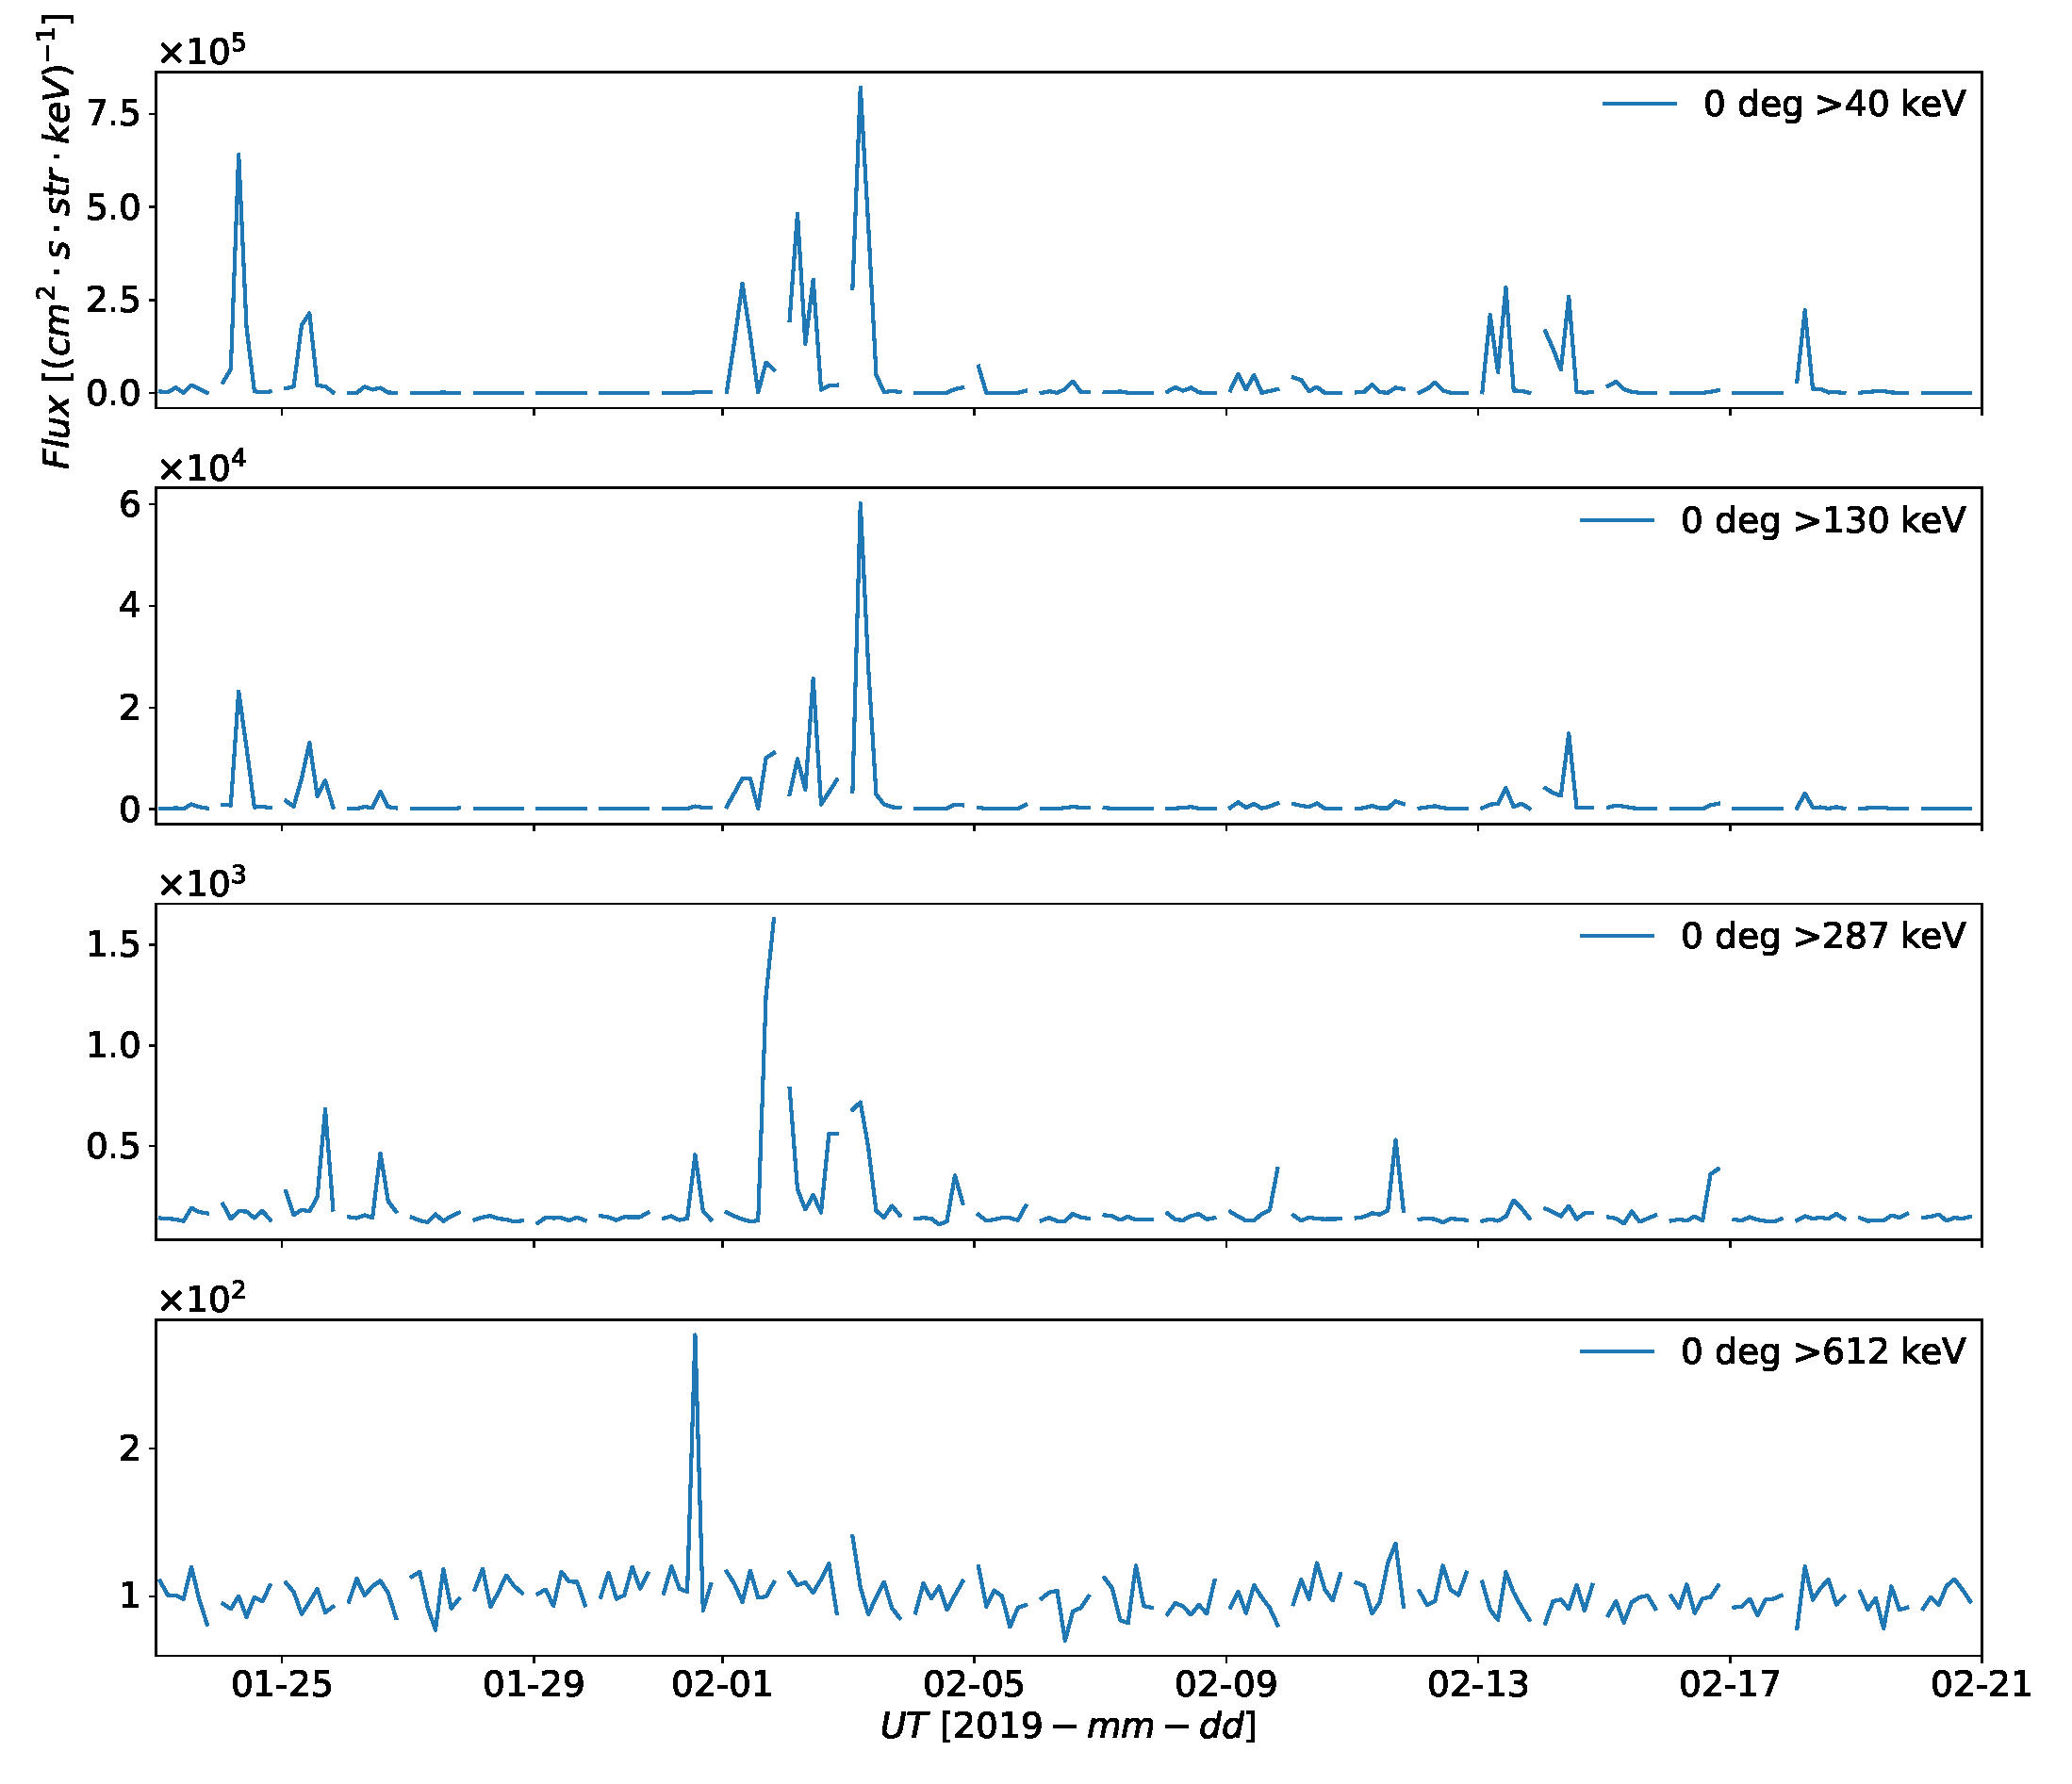
\includegraphics[width=\linewidth]{master_thesis_contents/master_thesis_fig/poes_tromsoe_0deg.pdf}
    \end{minipage}
    \caption{トロムソにおける柱密度(1段目。図\ref{fig:avg_ColumnDensity_tromsoe}と同じ)と電子フラックスデータ(2-5段目)との比較}
    \label{fig:ele_mmcd_tromsoe}
\end{figure}
\begin{figure}[htbp]
    \centering
    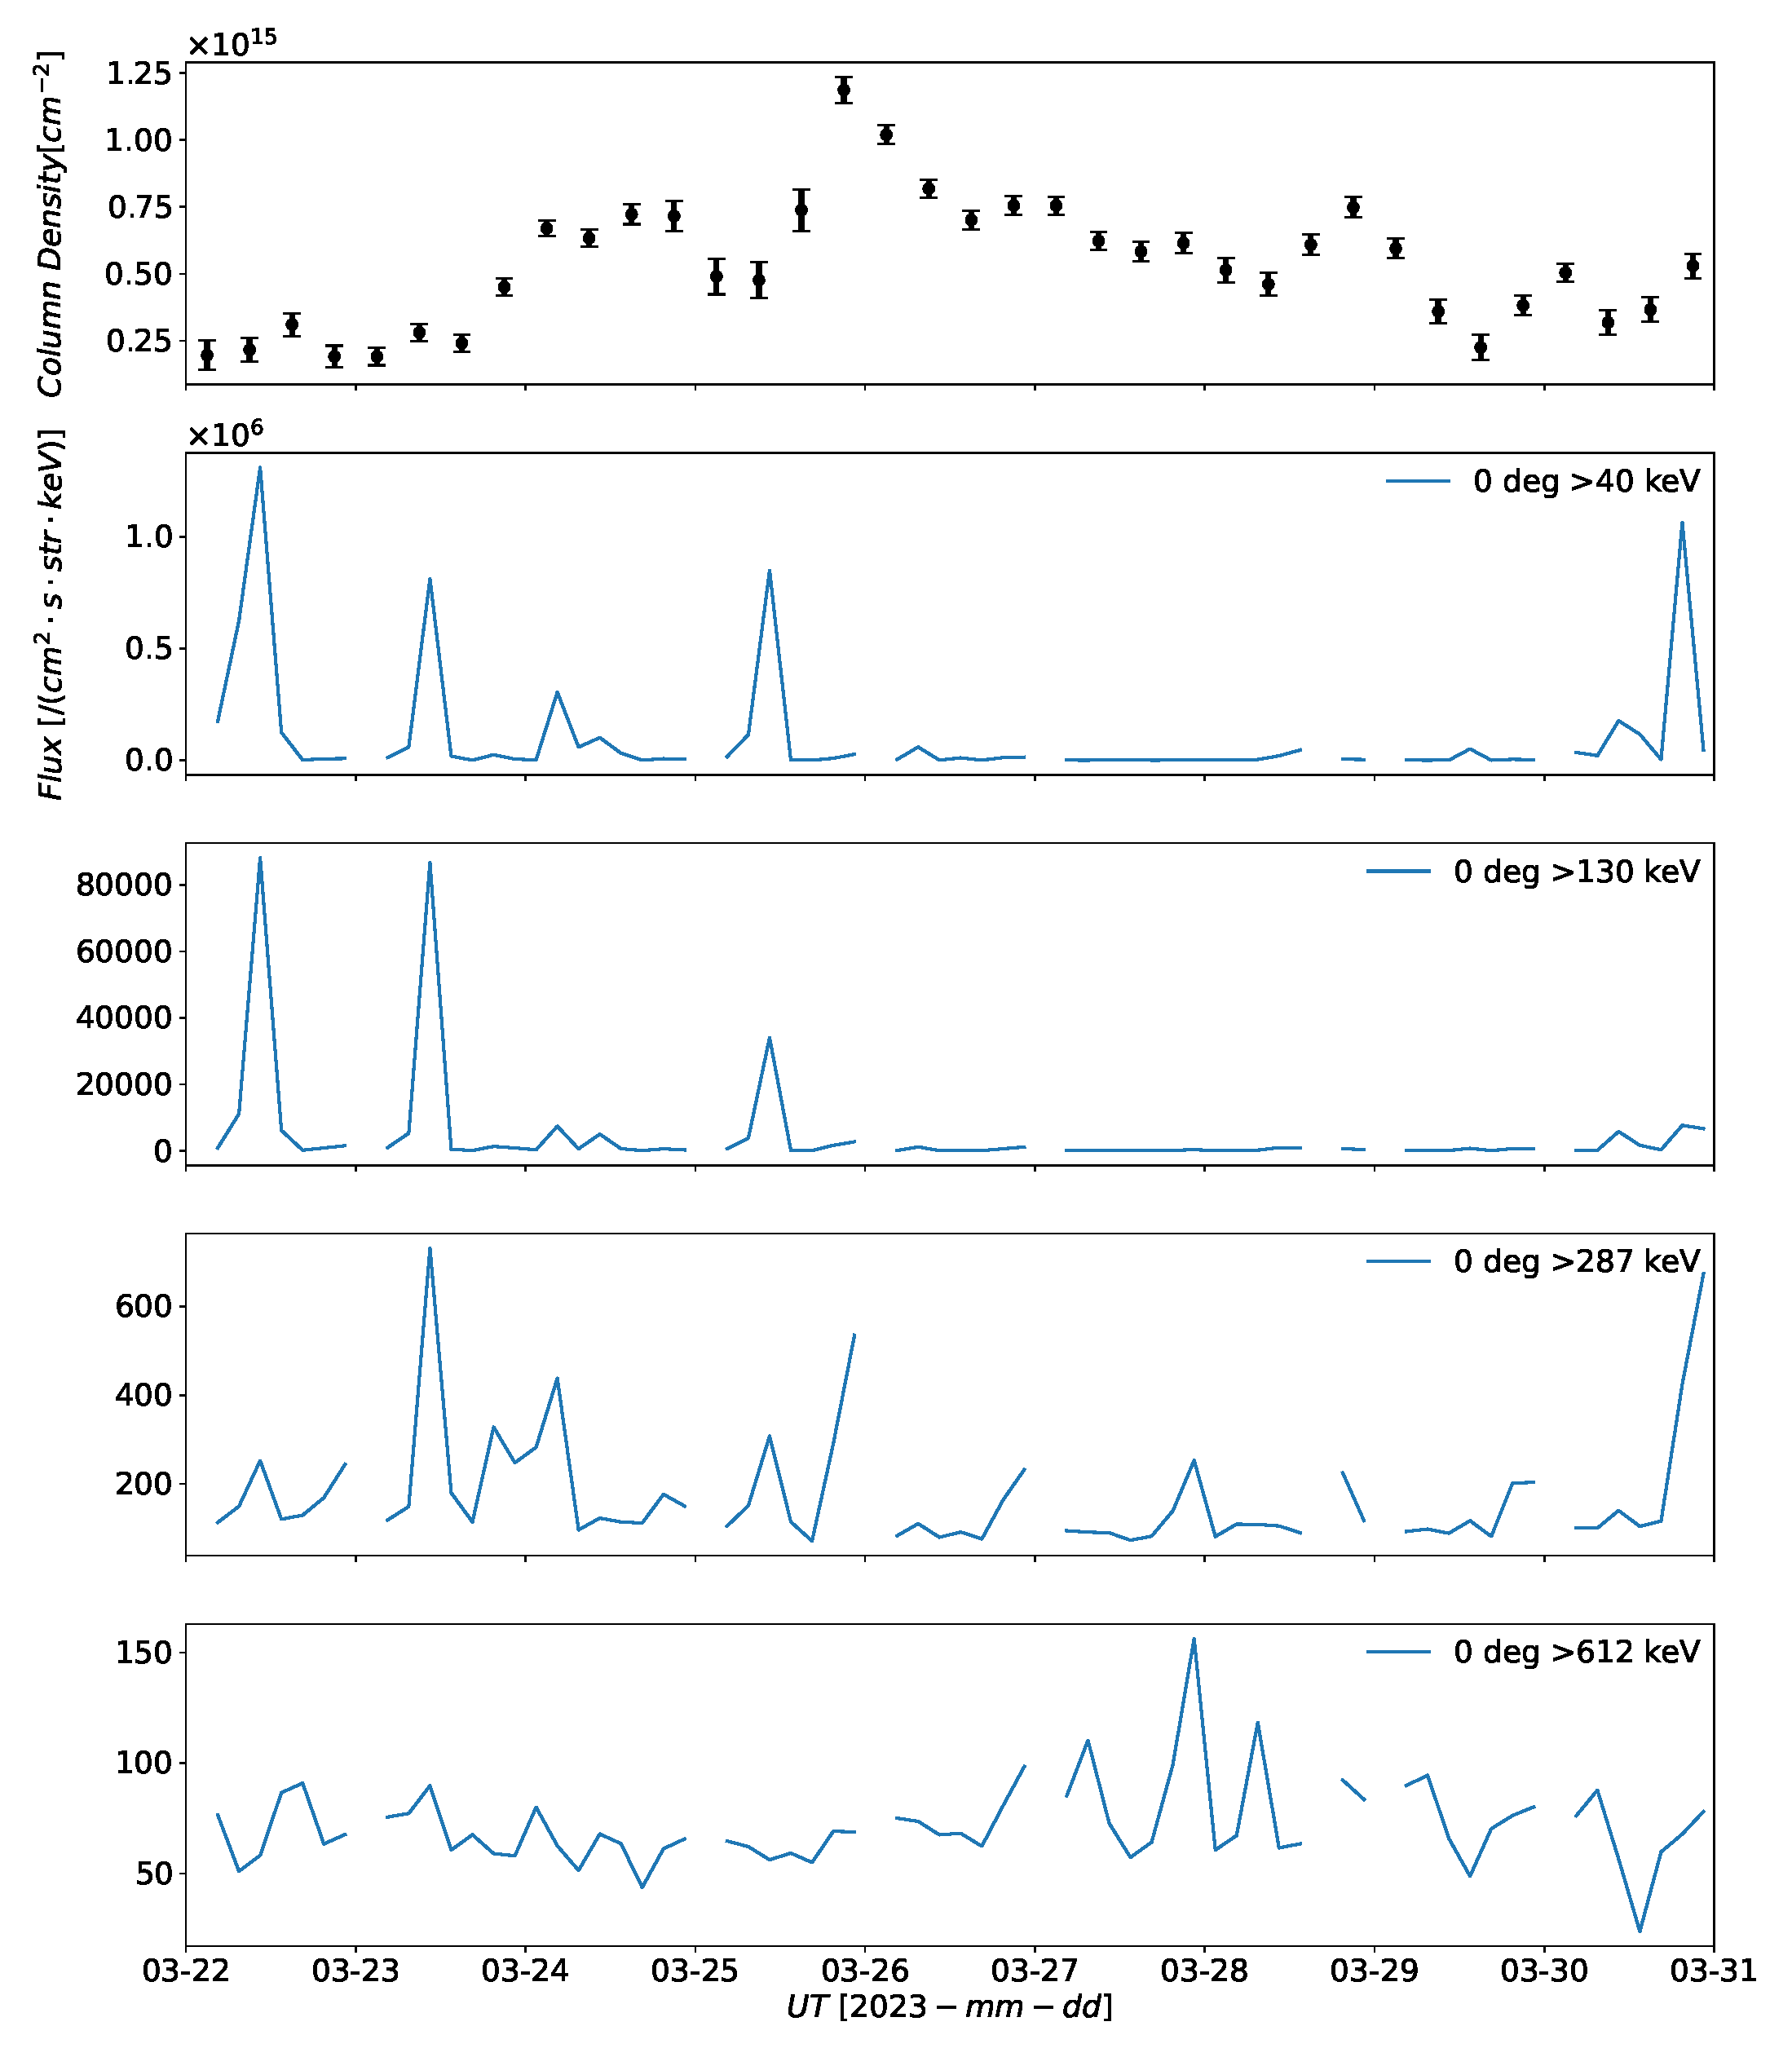
\includegraphics[width=\linewidth]{master_thesis_contents/master_thesis_fig/column_density_spectr6_poes0deg_syowa.pdf}
    \caption{昭和基地における柱密度(1段目。図\ref{fig:column_density_spectr6_syowa}と同じ)と電子フラックスデータ(2-5段目)との比較}
    \label{fig:ele_mmcd_syowa}
\end{figure}
\begin{figure}[htbp]
    \centering
    \begin{minipage}{\linewidth}
        \centering
        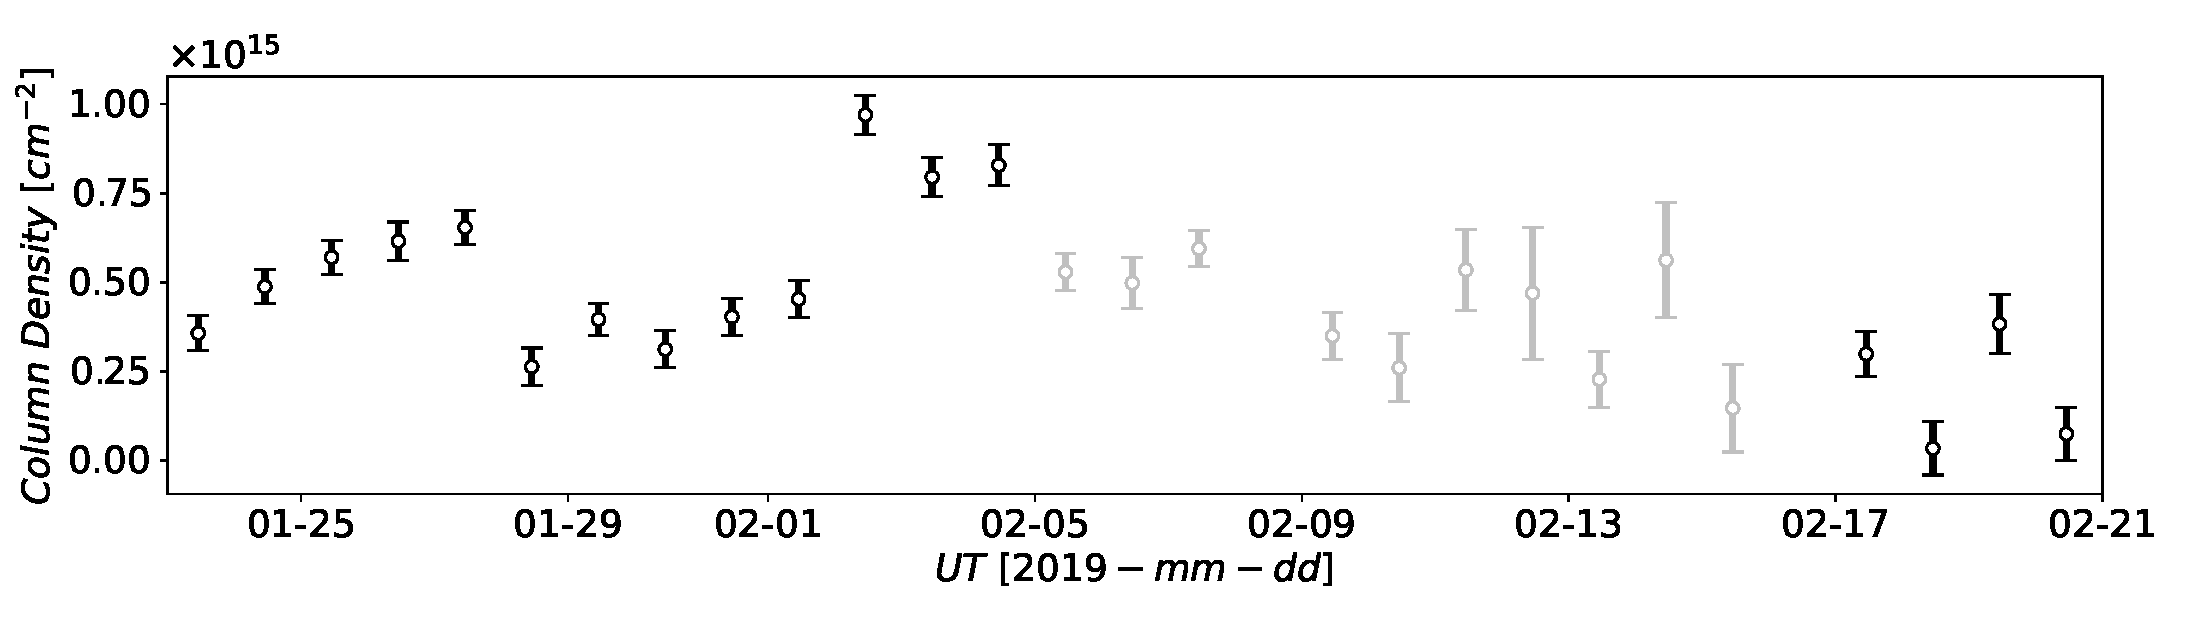
\includegraphics[width=\linewidth]{master_thesis_contents/master_thesis_fig/avg_ColumnDensity_tromsoe.pdf}
    \end{minipage}
    \begin{minipage}{\linewidth}
        \centering
        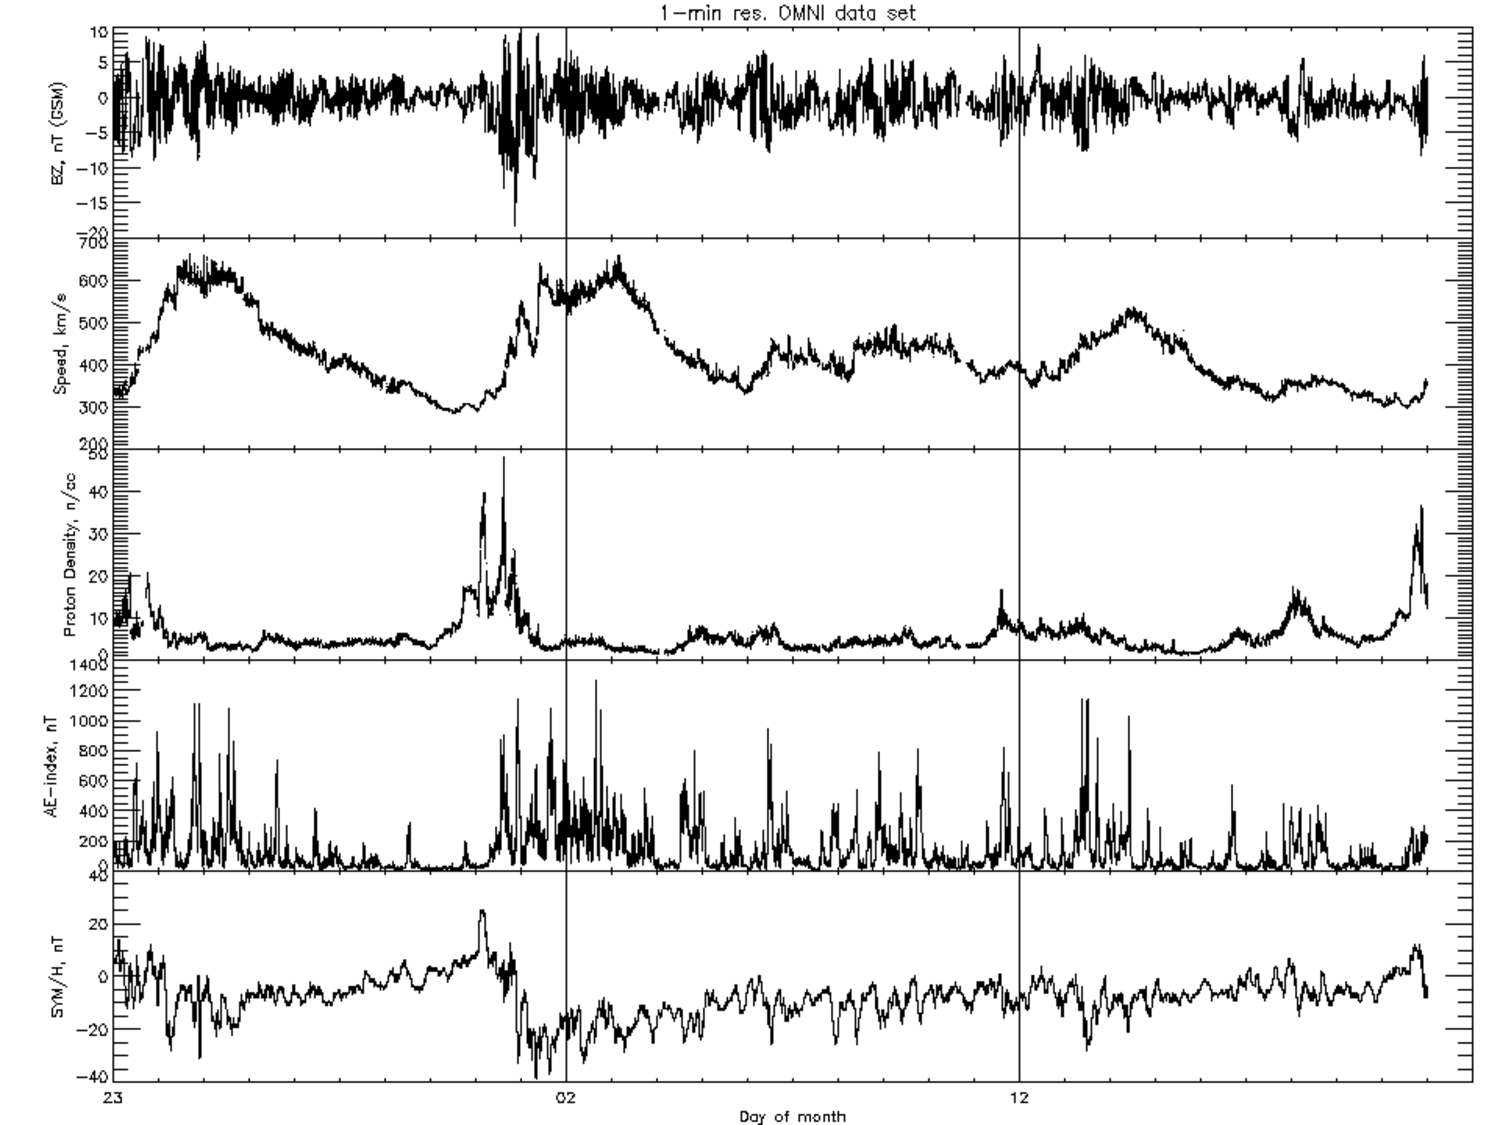
\includegraphics[width=\linewidth]{master_thesis_contents/master_thesis_fig/omni_tromsoe.pdf}
    \end{minipage}
    \caption{トロムソにおける柱密度(1段目。図\ref{fig:avg_ColumnDensity_tromsoe}と同じ)とOMNIデータ(2段目:地球磁場の南北成分、3段目:太陽風の速度、4段目:プロトン密度、5段目:AE指数、6段目:SYM/H)との比較}
    \label{fig:omni_mmcd_tromsoe}
\end{figure}
% 2つの図を整えて、揃えて出力する必要がある
% OMNIデータのAppendixを作る必要あり。
% SYM/HについてDst指数との関係を述べる。
\begin{figure}[htbp]
    \centering
    \begin{minipage}{\linewidth}
        \centering
        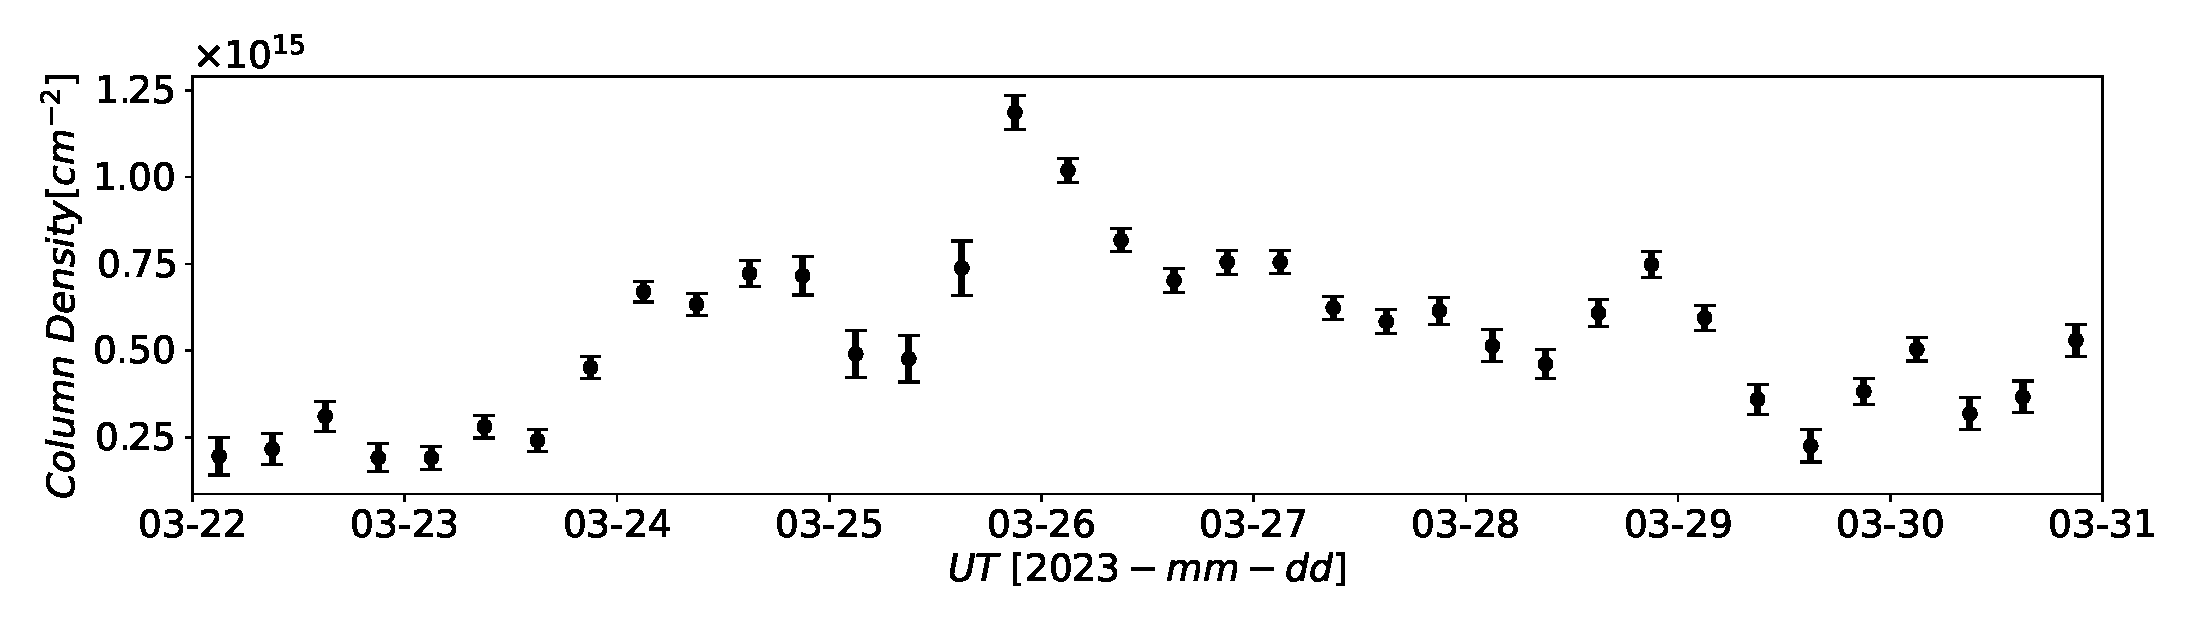
\includegraphics[width=\linewidth]{master_thesis_contents/master_thesis_fig/column_density_spectr6_syowa.pdf}
    \end{minipage}
    \begin{minipage}{0.96\linewidth}
        \centering
        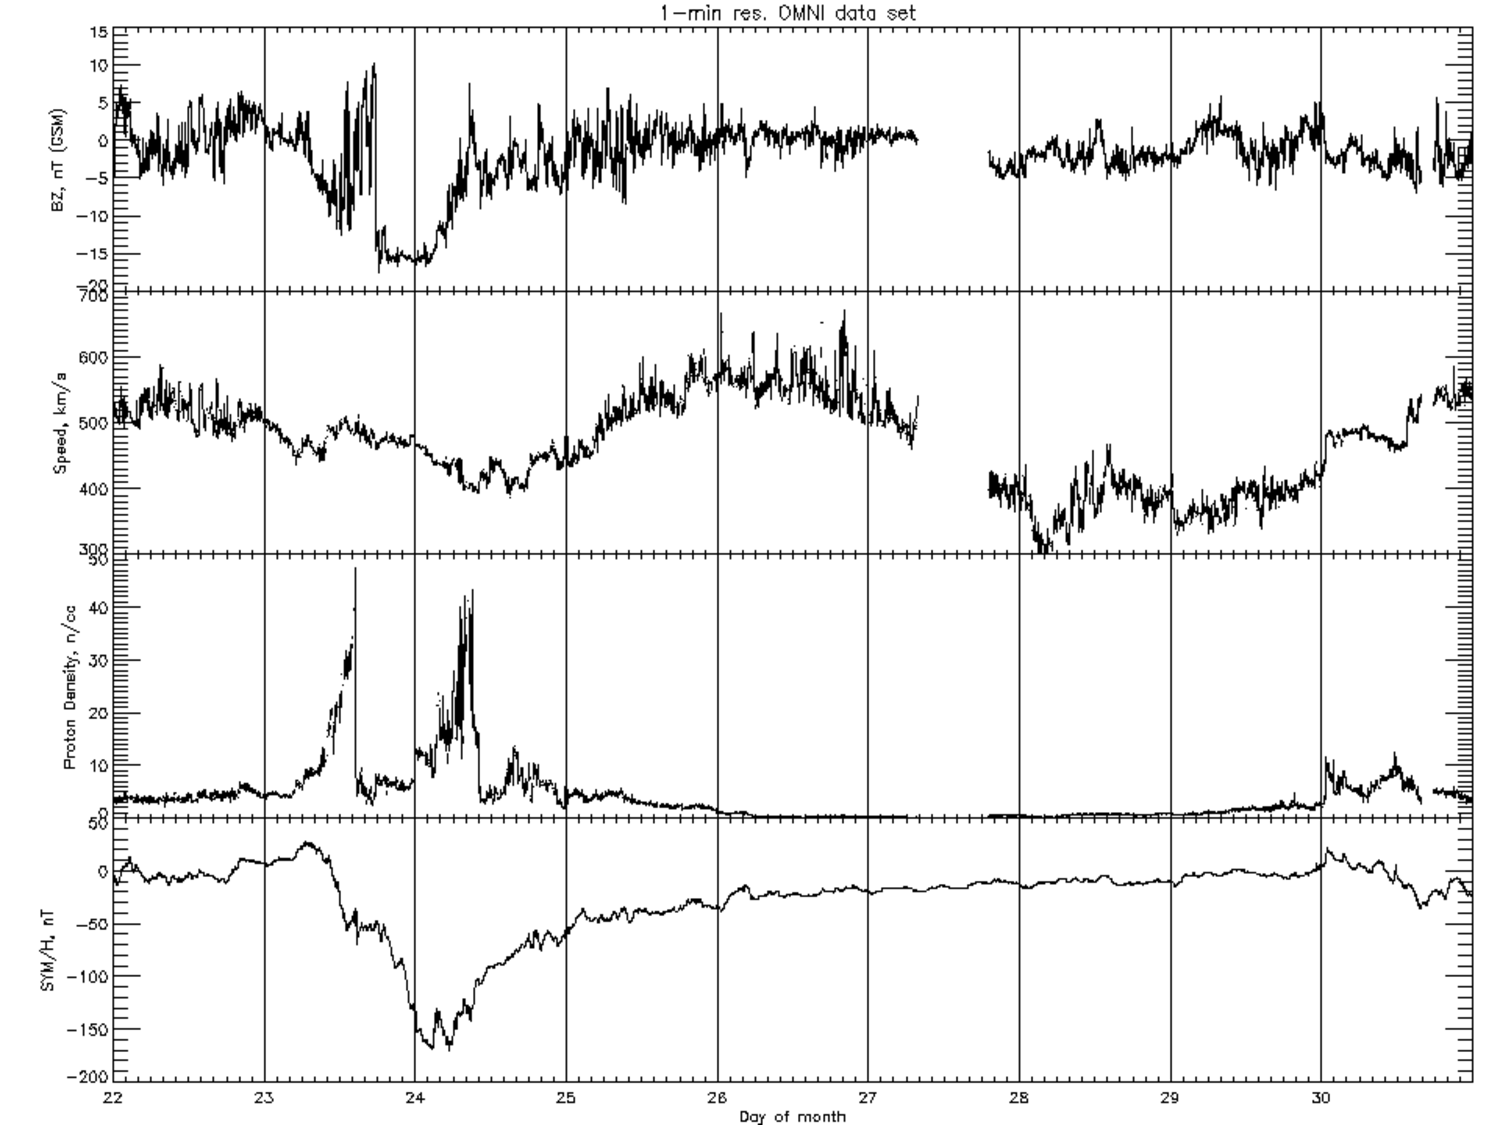
\includegraphics[width=\linewidth]{master_thesis_contents/master_thesis_fig/omni_syowa.pdf}
    \end{minipage}
    \caption{昭和基地における柱密度(1段目。図\ref{fig:avg_ColumnDensity_tromsoe}と同じ)とOMNIデータ(2段目:地球磁場の南北成分、3段目:太陽風の速度、4段目:プロトン密度、5段目:SYM/H)との比較}
    \label{fig:omni_mmcd_syowa}
\end{figure}
% 2つの図を整えて、揃えて出力する必要がある
% AE指数がない理由を述べる。


% \chapter{まとめ}
\chapter{まとめ}
% \label{ch:conclusion}
我々のグループでは、南極域だけでなく季節が逆転する北半球の極域にも着目し、両極域での比較観測を実現するために、実際に取得されたデータを精査して統一的な解析手法の開発を行った。
さらに、その時地球に降り込んできた高エネルギー粒子がどのように\ce{NO}分子の時間変動に影響を与えているかを調べた。
\par
本研究では、ミリ波分光計の仕様が異なる昭和基地とトロムソ両方のスペクトルデータの解析手法を検討した後、トロムソについては2018年12月26日から2019年3月10日までの75日間、昭和基地については2023年3月22日から31日までの10日間にわたる\ce{NO}の観測データの中から\ce{NO}の柱密度の導出を行って、その変動について考察した。
\par
トロムソの分光計では積分時間は24時間であったが、\ce{NO}の6本の超微細構造線から導出される柱密度を平均することで、昭和基地における積分時間は12時間と短くした。
昭和基地での柱密度の誤差の平均はトロムソでの観測と比べて20\% 小さくなり、時間分解能を小さくしながら柱密度の誤差を小さくすることができた。
解析の期間には磁場の擾乱により加速された電子の影響とみられる\ce{NO}の増加が確認できた。
\par
トロムソで観測されたミリ波分光による\ce{NO}の柱密度について、SOFIEによる衛星観測での\ce{NO}の密度に関する高度プロファイルデータから導出した柱密度と比較を行った結果、\ce{NO}の柱密度の時間変動について傾向が一致していることが分かった。
しかし、SOFIEから導出した\ce{NO}の柱密度は、ミリ波分光計から導出した\ce{NO}の柱密度と比べておよそ1.65倍されたものとなっていた。
これの原因の一部として、\ce{NO}の柱密度を導出する際に仮定した大気温度の値が妥当でない可能性があった。
ミリ波分光計を用いた\ce{NO}の柱密度の導出において仮定する大気温度の再検討をしたが、これだけで、SOFIEから導出した\ce{NO}の柱密度との値の差を説明することはできなかった。\ce{NO}の柱密度を導出する際には、大気温度を高度ごとに設定することも考慮に入れる必要がある。
また、POESによる衛星観測での電子フラックスデータの中でも、トロムソ・昭和基地付近に降り込むと考えられるデータを用いて、ミリ波分光による\ce{NO}の柱密度の時間変動と比較を行った。
電子フラックスの総量だけでなく、比較的エネルギーの大きい$>287\ \mathrm{keV}$における電子の増加量が\ce{NO}の増加の良い指標となることが明らかになった。
比較的エネルギーの小さい$>40\ \mathrm{keV}$, $>130\ \mathrm{keV}$の電子フラックスの増加があった期間では、顕著な\ce{NO}の増加がみられなかった。
\ce{NO}の柱密度の増加に寄与しない電子フラックスの増加の要因を探るため、磁気圏と電離層の様子を調べることができるOMNI Data Setを用いた比較を行った。
トロムソにおいては、\ce{NO}の柱密度の増加が確認された2つの時期どちらにおいても、地球磁場の南北成分のゆらぎがあり、サブストームが活発で高速太陽風が吹いていることが確認できた。
これらの影響により電子が加速され、\ce{NO}の増加につながったと考えられる。
昭和基地においては、磁気嵐の発生と対応して\ce{NO}の柱密度が増加した2023年3月23日〜2023年3月24日において地球磁場が南方向を向いており、プロトンの密度も上昇していることが確認できたが、高速太陽風は確認できなかった。
もう1つ柱密度の増加が確認できた2023年3月25日においては、SYM/H(もしくはDst指数)の値をみると磁気嵐は回復相にあたるが、高速太陽風があることが確認できた。
これは、高速太陽風の影響で電子が加速され\ce{NO}の増加につながった可能性が考えられる。


% \chapter*{謝辞}
\chapter*{謝辞}
% \label{ch:acknowledgement}


\bibliographystyle{junsrt}
\bibliography{ref}

\appendix
% \chapter{SOFIE衛星}
\chapter{SOFIE}
\label{app:sofie}
% (Solar Occultation for Ice Experiment)

% \chapter{POES/MetOp衛星}
\chapter{POES/MetOp}
\label{app:poes}
% (Polar Orbiting Environmental Satellites/Meteorological Operational Satellite)


\end{document}
